\chapter{中心极限定理}
\label{chap:central-limit-theorem}

把一枚均匀硬币掷$100$次，正面次数$S$的平均是$50$。大数律告诉我们，正面比例$S/100$会随掷的次数增多而靠近$1/2$；可是在$100$次这个具体的规模上，$S$不超过$55$的机会有多大？二项分布是已知的，把$56$个质量加起来，得到约$0.8644$。换一种算法：$S$的标准差是$5$，$55$比均值高出一个标准差，标准高斯分布在$1$处的分布函数值是$0.8413$；若把阈值取在$55.5$，得到$0.8643$，几乎与精确值重合。

钟形曲线为什么会出现在这里？硬币的每一次结果只取$0$和$1$，没有一点钟形的样子。原因在于$S$是$100$个独立小项之和：每一项单独都很粗糙，加起来以后，它们的细节互相抵消，留下的只有均值和方差。这就是\term{中心极限定理}（central limit theorem）所描述的现象：许多独立小扰动之和，中心化并按标准差缩放以后，分布逼近标准高斯分布。

这一章回答三个问题。第一，应当在什么尺度上观察波动：大数律说平均的偏差趋于零，偏差本身要放大多少倍才有稳定的形状。第二，什么条件保证放大后的形状是高斯的：独立同分布、各项分布不同、取值为向量，条件各有不同。第三，有限的样本量下，用高斯分布代替真实分布的误差有多大，又在哪些问题上不能这样代替。

全章以掷硬币的正面次数为主要例子，以指数分布的等待时间作为偏斜的对照。先确定标准化的中心和尺度，再在独立同分布情形用特征函数证明定理，然后放宽到三角阵和随机向量，最后用Berry--Esseen界估计正态近似的误差，并说明这个界管不到的地方。所用的弱收敛、特征函数及其连续性定理、Cramér--Wold判据都来自第~\ref{chap:weak-convergence-of-distributions}章。

\section{标准化波动}
\label{sec:clt-standardized}

掷$n$次硬币，我们可以看正面次数$S_n$，也可以看正面比例$\bar{X}_n=S_n/n$。两者只差一个因子$n$，可是随着$n$增大，一个越来越分散，一个越来越集中。要谈“波动的形状”，先得说清楚三件事：以什么为中心，看哪一个误差量，把误差放大多少倍。

第~\ref{chap:laws-of-large-numbers}章的大数律回答了中心的问题：样本平均趋于总体均值$\mu$，平均的偏差$\bar{X}_n-\mu$趋于零。它没有回答偏差以多快的速度缩小，也没有说明把偏差放大到合适的倍数以后是什么样子。本节先用方差确定合适的放大倍数，再说明标准化能做到什么、做不到什么。

\subsection{部分和与平均的尺度}
\label{sec:clt-scales}

设$X_1,X_2,\dots$独立同分布，均值为$\mu$，方差$\sigma^2$有限且大于零。记部分和与样本平均为
\[
 S_n=X_1+\dots+X_n,\qquad \bar{X}_n=\frac{S_n}{n} .
\]
两种误差量分别是部分和偏离$n\mu$的量$S_n-n\mu$，以及平均偏离$\mu$的量$\bar{X}_n-\mu$。

\paragraph{两种误差的方差}
独立随机变量之和的方差等于方差之和，常数平移不改变方差，所以
\[
 \operatorname{Var}(S_n-n\mu)=\sum_{i=1}^{n}\operatorname{Var}(X_i)=n\sigma^2 .
\]
再利用$\operatorname{Var}(aY)=a^2\operatorname{Var}(Y)$，取$a=1/n$，得到
\[
 \operatorname{Var}(\bar{X}_n-\mu)=\frac{1}{n^2}\cdot n\sigma^2=\frac{\sigma^2}{n} .
\]
两个结果合起来，标准差分别是
\begin{equation}
 \sqrt{\operatorname{Var}(S_n-n\mu)}=\sigma\sqrt{n},\qquad
 \sqrt{\operatorname{Var}(\bar{X}_n-\mu)}=\frac{\sigma}{\sqrt{n}} .
 \label{eq:clt-scales}
\end{equation}

部分和的典型偏差随$\sqrt{n}$增长，比$n$慢；平均的典型偏差随$1/\sqrt{n}$缩小，比$1/n$慢。前者慢于$n$，是因为独立的正负偏差互相抵消了一部分；后者慢于$1/n$，原因相同。把$n$项完全同向的偏差相加，标准差才会是$n\sigma$。

\paragraph{掷硬币}
设$X_i\sim\operatorname{Bern}(1/2)$，则$\mu=1/2$，$\sigma^2=1/4$，$S_n\sim\operatorname{Bin}(n,1/2)$。由式~\eqref{eq:clt-scales}，次数与比例的标准差分别为$\sqrt{n}/2$与$1/(2\sqrt{n})$。取$n=10,40,160$，
\[
 \frac{\sqrt{n}}{2}\approx1.58,\ 3.16,\ 6.32;\qquad \frac{1}{2\sqrt{n}}\approx0.158,\ 0.079,\ 0.040 .
\]
$n$每变成四倍，次数的标准差加倍，比例的标准差减半。

图~\ref{fig:clt-binomial-scales}画出这三个$n$下的精确质量表。左图以$n/2$为中心看次数，质量表随$n$摊开，峰值下降；右图以$1/2$为中心看比例，质量表向中心收拢。为了让不同$n$可比，右图的纵轴是质量除以格点间距$1/n$，这样曲线下的面积都是一。

\begin{BookInlineFigure}
 \centering
 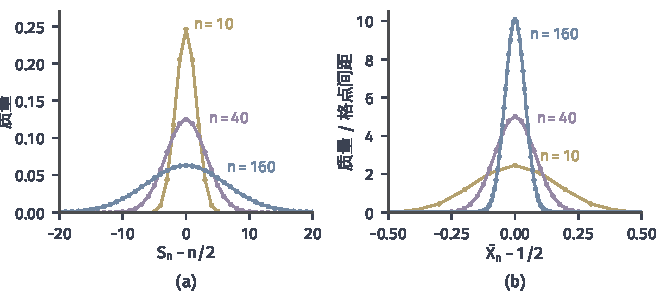
\includegraphics[width=112mm]{figures/07-probability/03-probability-limits/matplotlib/clt-binomial-scales/figure.pdf}
 \caption{均匀硬币掷$n$次的正面次数$S_n\sim\operatorname{Bin}(n,1/2)$，$n=10$（黄）、$40$（紫）、$160$（蓝），折线连接各格点上的精确质量。(a)中心化次数$S_n-n/2$的质量，宽度按$\sqrt{n}/2$增长；(b)中心化比例$\bar{X}_n-1/2$的质量除以格点间距$1/n$，宽度按$1/(2\sqrt{n})$缩小。}
 \label{fig:clt-binomial-scales}
\end{BookInlineFigure}

\paragraph{两种尺度不能混用}
这两个量回答不同的问题。问“正面次数偏离$n/2$不超过$5$次的概率”，随着$n$增大，这个概率趋于零，因为次数的典型偏差$\sqrt{n}/2$终将远超$5$。问“正面比例偏离$1/2$不超过$0.05$的概率”，它趋于一，这是大数律。两句话都对，只是固定的容许量$5$与$0.05$放在了不同的尺度上。

\paragraph{放大的倍数}
要得到不随$n$消失、也不随$n$发散的波动，可以把平均的偏差乘以$n^{a}$，看哪个$a$合适。由$\operatorname{Var}(cY)=c^2\operatorname{Var}(Y)$，
\[
 \operatorname{Var}\bigl(n^{a}(\bar{X}_n-\mu)\bigr)=n^{2a}\cdot\frac{\sigma^2}{n}=n^{2a-1}\sigma^2 .
\]
$a<1/2$时方差趋于零，由Chebyshev不等式，对每个$t>0$，
\[
 \mathbb{P}\bigl(\lvert n^{a}(\bar{X}_n-\mu)\rvert\geq t\bigr)\leq\frac{n^{2a-1}\sigma^2}{t^2}\to0 ,
\]
放大后的偏差依概率趋于零，形状缩成一点。$a>1/2$时方差趋于无穷，偏差越放越大。只有$a=1/2$时方差恒为$\sigma^2$。

图~\ref{fig:clt-three-scalings}用掷硬币的精确分布画出$a=0.3,0.5,0.7$三种放大下，中间$90\%$质量所在的区间随$n$的变化。三幅图的区间分别收窄、保持、扩张，紫色虚线是按方差预测的$\pm1.645\cdot\frac12 n^{a-1/2}$，其中$1.645$是标准高斯分布的$95\%$分位数。$a=1/2$时区间端点稳定在$\pm0.82$附近，与这条虚线吻合，这已经在提示极限分布是高斯的。

\begin{BookInlineFigure}
 \centering
 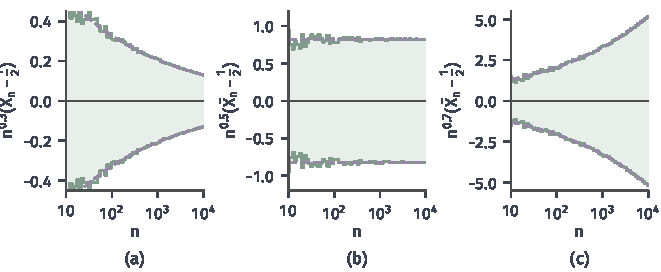
\includegraphics[width=112mm]{figures/07-probability/03-probability-limits/matplotlib/clt-three-scalings/figure.pdf}
 \caption{掷硬币时$n^{a}(\bar{X}_n-1/2)$的$5\%$与$95\%$分位数（绿色阶梯，由$\operatorname{Bin}(n,1/2)$精确计算），$n$从$10$到$10^{4}$，横轴为对数刻度。(a)$a=0.3$；(b)$a=0.5$；(c)$a=0.7$。紫色虚线为$\pm1.645\cdot\frac12n^{a-1/2}$。}
 \label{fig:clt-three-scalings}
\end{BookInlineFigure}

\paragraph{大数律与中心极限的分工}
大数律相当于取$a=0$：平均的偏差本身趋于零，它确定了极限的位置。中心极限定理研究$a=1/2$时放大后偏差的分布。前者不能推出后者：知道偏差趋于零，并不知道它以$1/\sqrt{n}$的速度趋于零，更不知道放大以后呈什么形状。下一小节会看到，平均同样趋于中心，放大后的形状却可以不是钟形。

方差无穷时，式~\eqref{eq:clt-scales}失去意义。例如第~\ref{chap:tail-probabilities}章参数为$3/2$的Pareto分布，均值有限，样本平均仍满足大数律，方差却是无穷，$\sqrt{n}$不再是合适的放大倍数。本章始终假设方差有限，这类重尾的极限需要别的尺度，不在本卷讨论。

\subsection{标准化的选择}
\label{sec:clt-standardization}

确定了放大倍数$\sqrt{n}$，再除以单项的标准差，就把波动的单位也去掉了。由式~\eqref{eq:clt-scales}，中心化部分和除以它自己的标准差，与平均的偏差乘$\sqrt{n}$再除以$\sigma$，是同一个量。

\begin{definition}[标准化部分和]
\label{def:clt-standardized-sum}
设$X_1,\dots,X_n$独立同分布，均值为$\mu$，方差$\sigma^2\in(0,\infty)$。称
\begin{equation}
 Z_n=\frac{S_n-n\mu}{\sigma\sqrt{n}}=\frac{\sqrt{n}\,(\bar{X}_n-\mu)}{\sigma}
 \label{eq:clt-zn}
\end{equation}
为标准化部分和。
\end{definition}

$Z_n$正是第~\ref{chap:random-variable-moments}章意义下$S_n$的标准化，也是$\bar{X}_n$的标准化：两者只差一个正的倍数，标准化后相同。由式~\eqref{eq:clt-scales}，对每个$n$都有
\[
 \mathbb{E}[Z_n]=0,\qquad \operatorname{Var}(Z_n)=1 .
\]
掷硬币时$\mu=1/2$，$\sigma=1/2$，于是$Z_n=(2S_n-n)/\sqrt{n}$。$n=100$时$Z_{100}=(S_{100}-50)/5$，章首的阈值$55$对应$Z_{100}=1$。

\paragraph{方差为一不等于钟形}
标准化只做平移和正的缩放，不改变分布的形状。$n=1$时$Z_1$就是$X_1$的标准化，硬币的$Z_1$只取$\pm1$两个值，与钟形毫无关系。$Z_n$接近钟形，是因为$S_n$是许多独立项之和，不是因为除以了标准差。

即使项数很多，标准化也不能保证钟形。设第$n$次试验掷$n$枚特制的硬币，每枚正面的概率是$1/n$，正面总数$S_n\sim\operatorname{Bin}(n,1/n)$。它的均值和方差是
\[
 \mathbb{E}[S_n]=1,\qquad \operatorname{Var}(S_n)=n\cdot\frac1n\Bigl(1-\frac1n\Bigr)=1-\frac1n .
\]
平均$S_n/n$同样趋于零，标准化以后均值为零、方差为一。可是$S_n$只取非负整数，它的前几个质量趋于
\[
 \mathbb{P}(S_n=0)=\Bigl(1-\frac1n\Bigr)^{n}\to\mathrm{e}^{-1}\approx0.368,\qquad
 \mathbb{P}(S_n=1)=\Bigl(1-\frac1n\Bigr)^{n-1}\to\mathrm{e}^{-1} .
\]
一般地，第~\ref{chap:common-distributions}章已经说明$\operatorname{Bin}(n,\lambda/n)$的质量趋于$\operatorname{Poisson}(\lambda)$的质量，这里$\lambda=1$，所以$S_n-1$的分布逼近$\operatorname{Poisson}(1)$平移$-1$后的分布。

图~\ref{fig:clt-poisson-counter}把这两种标准化计数放在一起。左边是$\operatorname{Bin}(100,1/2)$，格点间距$1/5$，质量除以间距后贴着标准高斯密度$\varphi$；右边是$\operatorname{Bin}(100,1/100)$，标准化以后只有几根竖线，集中在$z=-1,0,1,2$附近，没有平滑的钟形。

\begin{BookInlineFigure}
 \centering
 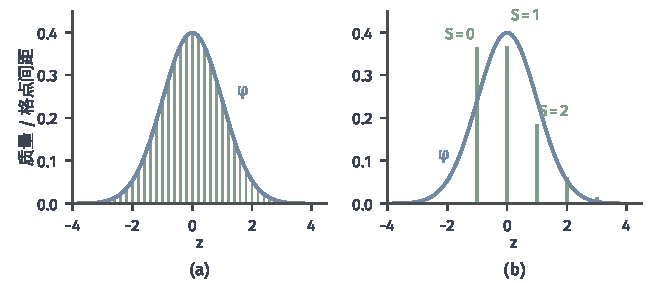
\includegraphics[width=112mm]{figures/07-probability/03-probability-limits/matplotlib/clt-poisson-counter/figure.pdf}
 \caption{两个$n=100$的标准化二项计数，均值都为$0$、方差都为$1$。绿色竖线是精确质量除以格点间距$1/\sigma_n$，蓝线是标准高斯密度$\varphi$。(a)$\operatorname{Bin}(100,1/2)$，$\sigma_n=5$；(b)$\operatorname{Bin}(100,1/100)$，$\sigma_n\approx0.995$，质量集中在$S=0,1,2$等少数格点。}
 \label{fig:clt-poisson-counter}
\end{BookInlineFigure}

两种计数的差别在于每一项对总和的影响。正面概率为$1/2$时，每枚硬币只贡献总方差的$1/n$，没有哪一枚举足轻重；正面概率为$1/n$时，总和几乎由“偶尔出现的一次正面”决定，这样一次正面就让$S_n$跳动一个标准差。第~\ref{sec:clt-non-identical}节会把“没有一项举足轻重”写成可以核验的条件。

\paragraph{零方差}
定义~\ref{def:clt-standardized-sum}要求$\sigma^2>0$。若$\sigma^2=0$，则$X_i$以概率一等于$\mu$，部分和$S_n-n\mu$以概率一为零，没有波动可言，也不能除以$\sigma$。此时不作标准化，直接说$\sqrt{n}(\bar{X}_n-\mu)$以概率一等于零，它的分布是$0$处的单点分布。把方差为零的高斯分布$\mathcal{N}(0,0)$理解为这个单点分布，零方差情形也可以纳入第~\ref{sec:clt-multivariate}节的统一陈述。


\section{独立同分布情形}
\label{sec:clt-iid}

标准化部分和$Z_n$的均值和方差已经固定为$0$和$1$，上一节也看到，形状要靠“许多独立的小项”才会变成钟形。最简单的情形是各项来自同一个分布：每一项对总和的贡献都是总方差的$1/n$，没有哪一项占优。本节在这个情形下陈述并证明中心极限定理，只要求方差有限。

\subsection{定理与条件}
\label{sec:clt-iid-theorem}

先看一个偏斜得很厉害的例子。设$X_i\sim\operatorname{Exp}(1)$独立，表示一串相互独立的等待时间，$\mu=\sigma=1$。由第~\ref{chap:random-variable-transformations}章的卷积计算，$S_n\sim\operatorname{Gamma}(n,1)$，所以$Z_n=(S_n-n)/\sqrt{n}$的密度可以精确写出：
\[
 f_{Z_n}(z)=\sqrt{n}\,f_{S_n}(n+z\sqrt{n}),\qquad f_{S_n}(s)=\frac{s^{n-1}\mathrm{e}^{-s}}{(n-1)!}\ (s>0) .
\]
这里用了第~\ref{chap:random-variable-transformations}章的一元换元：$Z_n$是$S_n$的仿射函数，密度要乘以斜率的倒数$\sqrt{n}$。

图~\ref{fig:clt-gamma-densities}画出$n=1,4,16$时的$f_{Z_n}$。$n=1$时它是平移后的指数密度，在$z=-1$处突然跳起，右侧拖着长尾；$n=4$时已经有了圆顶，但峰偏在左边；$n=16$时与标准高斯密度只差一点偏斜。偏斜的程度可以用偏度衡量，$\operatorname{Gamma}(n,1)$的偏度是$2/\sqrt{n}$，按$1/\sqrt{n}$消失。

\begin{BookInlineFigure}
 \centering
 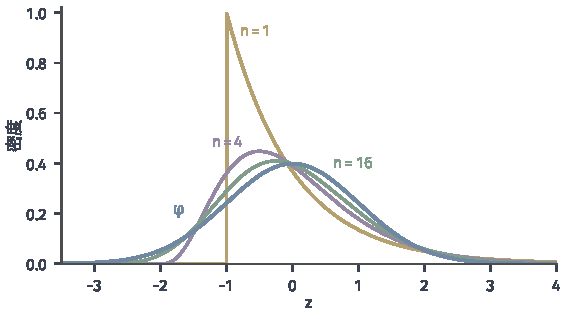
\includegraphics[width=96mm]{figures/07-probability/03-probability-limits/matplotlib/clt-gamma-densities/figure.pdf}
 \caption{$n$个独立$\operatorname{Exp}(1)$之和的标准化$Z_n=(S_n-n)/\sqrt{n}$的精确密度，$n=1$（黄）、$4$（紫）、$16$（绿），蓝线为标准高斯密度$\varphi$。$n=1$时密度在$z=-1$处从$0$跳到$1$。}
 \label{fig:clt-gamma-densities}
\end{BookInlineFigure}

硬币与等待时间的单项分布截然不同，一个只取两个值，一个是连续的偏斜密度，标准化和却都趋于同一个形状。下面的定理说，只要独立、同分布、方差有限且为正，这个现象总会发生。

\begin{theorem}[独立同分布的中心极限定理]
\label{thm:clt-iid}
设$X_1,X_2,\dots$独立同分布，$\mathbb{E}[X_1]=\mu$，$\operatorname{Var}(X_1)=\sigma^2\in(0,\infty)$，$Z_n$如式~\eqref{eq:clt-zn}。则
\begin{equation}
 Z_n=\frac{S_n-n\mu}{\sigma\sqrt{n}}\xrightarrow{\mathrm{d}}\mathcal{N}(0,1) .
 \label{eq:clt-iid}
\end{equation}
\end{theorem}

\paragraph{用分布函数表述}
标准高斯分布函数$\Phi$处处连续，没有需要排除的跳点。由第~\ref{chap:weak-convergence-of-distributions}章的分布函数判据，式~\eqref{eq:clt-iid}等价于对每个实数$x$，
\begin{equation}
 \mathbb{P}(Z_n\leq x)\to\Phi(x) .
 \label{eq:clt-iid-cdf}
\end{equation}
于是对任意$a<b$，$\mathbb{P}(a<Z_n\leq b)\to\Phi(b)-\Phi(a)$。端点是否取等号不影响极限：$\mathbb{P}(Z_n=x)\leq\mathbb{P}(x-\eta<Z_n\leq x)$对每个$\eta>0$成立，右边趋于$\Phi(x)-\Phi(x-\eta)$，可以任意小。

把定理用于$X_i\sim\operatorname{Bern}(p)$，$0<p<1$，就得到二项计数的正态逼近：
\[
 \frac{S_n-np}{\sqrt{np(1-p)}}\xrightarrow{\mathrm{d}}\mathcal{N}(0,1),\qquad S_n\sim\operatorname{Bin}(n,p) .
\]
这个特例称为\term{de Moivre--Laplace定理}（de Moivre--Laplace theorem），它是中心极限定理最早的形式。

\paragraph{各个条件的作用}
定理有三个条件。独立性使和的特征函数能拆成乘积，这是证明的起点；同分布使每个因子相同，$n$个小贡献完全对称；方差有限且为正，既给出了标准化的尺度，也保证下面的二阶展开成立。上一节的特制硬币各项分布随$n$变化，不在定理的范围里，它的极限也确实不是高斯的。

定理只要求二阶矩有限，不要求三阶矩，也不要求矩母函数存在。第~\ref{sec:clt-error}节估计近似误差时要用三阶绝对矩，那是为了得到收敛的速度，不是收敛本身的条件。第~\ref{chap:weak-convergence-of-distributions}章说明过，矩母函数可能在零点附近的任何邻域都无穷，而特征函数总是存在，所以证明用特征函数。

\subsection{特征函数证明}
\label{sec:clt-iid-proof}

把$X_i$标准化，令$Y_i=(X_i-\mu)/\sigma$。$Y_i$独立同分布，$\mathbb{E}[Y_i]=0$，$\mathbb{E}[Y_i^2]=1$，并且
\[
 Z_n=\frac{1}{\sqrt{n}}\sum_{i=1}^{n}Y_i .
\]
记$Y$为与$Y_i$同分布的变量，$\phi_Y$为它的特征函数。第~\ref{chap:weak-convergence-of-distributions}章给出了两条运算规则：数乘满足$\phi_{cY}(t)=\phi_Y(ct)$；独立变量之和的特征函数是各自特征函数的乘积。合起来，
\begin{equation}
 \phi_{Z_n}(t)=\prod_{i=1}^{n}\phi_{Y_i}\Bigl(\frac{t}{\sqrt{n}}\Bigr)=\phi_Y\Bigl(\frac{t}{\sqrt{n}}\Bigr)^{n} .
 \label{eq:clt-product}
\end{equation}
标准高斯分布的特征函数是$\mathrm{e}^{-t^2/2}$，由连续性定理，只需证明式~\eqref{eq:clt-product}对每个$t$趋于$\mathrm{e}^{-t^2/2}$。

\paragraph{为什么会出现$\mathrm{e}^{-t^2/2}$}
先用直觉看一遍。$t/\sqrt{n}$很小，$\phi_Y$在原点附近的展开是
\[
 \phi_Y(s)=\mathbb{E}[\mathrm{e}^{\mathrm{i}sY}]\approx1+\mathrm{i}s\,\mathbb{E}[Y]-\frac{s^2}{2}\mathbb{E}[Y^2]=1-\frac{s^2}{2} .
\]
代入$s=t/\sqrt{n}$再取$n$次方，
\[
 \phi_{Z_n}(t)\approx\Bigl(1-\frac{t^2}{2n}\Bigr)^{n}\to\mathrm{e}^{-t^2/2} .
\]
中心化让一次项消失，方差为一让二次项的系数是$1/2$。剩下要说明的是：被“$\approx$”丢掉的余项乘上$n$个因子以后，累计起来仍然可以忽略。

第~\ref{chap:weak-convergence-of-distributions}章在二阶矩有限时给出了上面的展开，余项是$s^2$的高阶无穷小。为了在$n$个因子的乘积里累计余项，我们把余项写成显式的界，下面两个引理分别处理单个因子和乘积。

\begin{lemma}[复指数的二阶展开]
\label{lem:clt-exp-remainder}
对每个实数$x$，
\begin{equation}
 \Bigl\lvert\mathrm{e}^{\mathrm{i}x}-1-\mathrm{i}x+\frac{x^2}{2}\Bigr\rvert\leq\min\Bigl\{\frac{\lvert x\rvert^{3}}{6},\ x^2\Bigr\} .
 \label{eq:clt-exp-remainder}
\end{equation}
\end{lemma}

\begin{proof}
对积分$\int_0^x(x-u)\mathrm{e}^{\mathrm{i}u}\,\mathrm{d}u$分部积分，取$\mathrm{e}^{\mathrm{i}u}$的原函数$-\mathrm{i}\mathrm{e}^{\mathrm{i}u}$，得到
\[
 \int_0^x(x-u)\mathrm{e}^{\mathrm{i}u}\,\mathrm{d}u
 =\Bigl[-\mathrm{i}(x-u)\mathrm{e}^{\mathrm{i}u}\Bigr]_0^x-\mathrm{i}\int_0^x\mathrm{e}^{\mathrm{i}u}\,\mathrm{d}u
 =\mathrm{i}x-(\mathrm{e}^{\mathrm{i}x}-1) .
\]
移项得到一次展开的余项公式
\[
 \mathrm{e}^{\mathrm{i}x}-1-\mathrm{i}x=-\int_0^x(x-u)\mathrm{e}^{\mathrm{i}u}\,\mathrm{d}u .
\]

第一个界。$x^2/2=\int_0^x(x-u)\,\mathrm{d}u$，与上式相加，
\[
 \mathrm{e}^{\mathrm{i}x}-1-\mathrm{i}x+\frac{x^2}{2}=\int_0^x(x-u)\bigl(1-\mathrm{e}^{\mathrm{i}u}\bigr)\,\mathrm{d}u .
\]
被积函数中$\lvert1-\mathrm{e}^{\mathrm{i}u}\rvert\leq2$，$x-u$在积分区间上不变号，所以
\[
 \Bigl\lvert\mathrm{e}^{\mathrm{i}x}-1-\mathrm{i}x+\frac{x^2}{2}\Bigr\rvert\leq2\Bigl\lvert\int_0^x(x-u)\,\mathrm{d}u\Bigr\rvert=x^2 .
\]

第二个界。再对$\int_0^x(x-u)^2\mathrm{e}^{\mathrm{i}u}\,\mathrm{d}u$分部积分，并代入前面的结果：
\[
 \int_0^x(x-u)^2\mathrm{e}^{\mathrm{i}u}\,\mathrm{d}u
 =\mathrm{i}x^2-2\mathrm{i}\int_0^x(x-u)\mathrm{e}^{\mathrm{i}u}\,\mathrm{d}u
 =\mathrm{i}x^2-2\mathrm{i}\bigl(1+\mathrm{i}x-\mathrm{e}^{\mathrm{i}x}\bigr) .
\]
两边除以$2\mathrm{i}$并整理，
\[
 \mathrm{e}^{\mathrm{i}x}-1-\mathrm{i}x+\frac{x^2}{2}=\frac{1}{2\mathrm{i}}\int_0^x(x-u)^2\mathrm{e}^{\mathrm{i}u}\,\mathrm{d}u .
\]
被积函数的模是$(x-u)^2$，所以
\[
 \Bigl\lvert\mathrm{e}^{\mathrm{i}x}-1-\mathrm{i}x+\frac{x^2}{2}\Bigr\rvert\leq\frac12\Bigl\lvert\int_0^x(x-u)^2\,\mathrm{d}u\Bigr\rvert=\frac{\lvert x\rvert^3}{6} .
\]
\end{proof}

两个界各管一段，见图~\ref{fig:clt-remainder}。$\lvert x\rvert$小的时候，三次界$\lvert x\rvert^3/6$更小，余项确实是三阶小量；$\lvert x\rvert$大的时候，二次界$x^2$更小，因为余项最多和$x^2/2$同阶，不会像$\lvert x\rvert^3$那样增长。两条界在$\lvert x\rvert=6$处相交。证明中正是要用后一个界：$Y$只有二阶矩，$\mathbb{E}[\lvert Y\rvert^3]$可能是无穷，但$\mathbb{E}[Y^2]$一定有限。

\begin{BookInlineFigure}
 \centering
 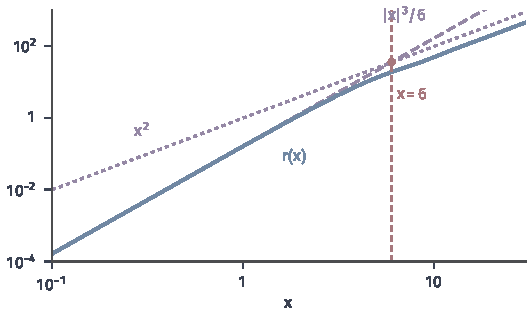
\includegraphics[width=90mm]{figures/07-probability/03-probability-limits/matplotlib/clt-remainder/figure.pdf}
 \caption{二阶展开的余项$r(x)=\lvert\mathrm{e}^{\mathrm{i}x}-1-\mathrm{i}x+x^2/2\rvert$（蓝）与两条上界$\lvert x\rvert^3/6$（紫色虚线）、$x^2$（紫色点线），双对数坐标。两条界在$x=6$（红点）相交，$x<6$时三次界更紧，$x>6$时二次界更紧。}
 \label{fig:clt-remainder}
\end{BookInlineFigure}

\begin{lemma}[乘积之差]
\label{lem:clt-product-difference}
设复数$z_1,\dots,z_m$与$w_1,\dots,w_m$的模都不超过$1$。则
\begin{equation}
 \Bigl\lvert\prod_{k=1}^{m}z_k-\prod_{k=1}^{m}w_k\Bigr\rvert\leq\sum_{k=1}^{m}\lvert z_k-w_k\rvert .
 \label{eq:clt-product-difference}
\end{equation}
\end{lemma}

\begin{proof}
对$m$归纳。$m=1$时两边相等。设结论对$m-1$成立，记$P=\prod_{k<m}z_k$，$Q=\prod_{k<m}w_k$，它们的模不超过$1$。拆开差，
\[
 Pz_m-Qw_m=z_m(P-Q)+(z_m-w_m)Q .
\]
由$\lvert z_m\rvert\leq1$与$\lvert Q\rvert\leq1$，
\[
 \lvert Pz_m-Qw_m\rvert\leq\lvert P-Q\rvert+\lvert z_m-w_m\rvert ,
\]
再对$\lvert P-Q\rvert$用归纳假设即得。
\end{proof}

这个引理说，模不超过一的因子相乘时，各因子的误差至多简单相加，不会被放大。所以只要每个因子的误差是$o(1/n)$，$n$个因子的累计误差就是$o(1)$。

\begin{proof}[定理~\ref{thm:clt-iid}的证明]
固定$t$，记$s=t/\sqrt{n}$。

第一步，单个因子的误差。在式~\eqref{eq:clt-exp-remainder}中令$x=sY$，取期望。由$\mathbb{E}[Y]=0$，$\mathbb{E}[Y^2]=1$，左边期望里的各项分别给出$\phi_Y(s)$、$1$、$0$和$s^2/2$；再用“期望的模不超过模的期望”，得到
\[
 \Bigl\lvert\phi_Y(s)-\Bigl(1-\frac{s^2}{2}\Bigr)\Bigr\rvert
 \leq\mathbb{E}\Bigl[\min\Bigl\{\frac{\lvert s\rvert^{3}\lvert Y\rvert^{3}}{6},\ s^2Y^2\Bigr\}\Bigr] .
\]
代入$s=t/\sqrt{n}$，两边乘$n$，
\[
 n\Bigl\lvert\phi_Y\Bigl(\frac{t}{\sqrt{n}}\Bigr)-\Bigl(1-\frac{t^2}{2n}\Bigr)\Bigr\rvert
 \leq t^2\,\mathbb{E}\Bigl[\min\Bigl\{\frac{\lvert t\rvert\,\lvert Y\rvert^{3}}{6\sqrt{n}},\ Y^2\Bigr\}\Bigr] .
\]

第二步，右边趋于零。期望里的随机变量对每个样本点都趋于零，因为$\lvert Y\rvert^3/\sqrt{n}\to0$；它又被可积的$Y^2$控制。由支配收敛定理，右边的期望趋于零。这里只用到$\mathbb{E}[Y^2]<\infty$。

第三步，累计。$n\geq t^2/2$时，$\lvert1-t^2/(2n)\rvert\leq1$；特征函数的模也不超过$1$。对式~\eqref{eq:clt-product}的$n$个因子用引理~\ref{lem:clt-product-difference}，
\[
 \Bigl\lvert\phi_{Z_n}(t)-\Bigl(1-\frac{t^2}{2n}\Bigr)^{n}\Bigr\rvert
 \leq n\Bigl\lvert\phi_Y\Bigl(\frac{t}{\sqrt{n}}\Bigr)-\Bigl(1-\frac{t^2}{2n}\Bigr)\Bigr\rvert\to0 .
\]

第四步，极限。由$\ln(1-y)/y\to-1$（$y\to0$），$n\ln(1-t^2/(2n))\to-t^2/2$，所以
\[
 \Bigl(1-\frac{t^2}{2n}\Bigr)^{n}\to\mathrm{e}^{-t^2/2} .
\]
两步合起来，$\phi_{Z_n}(t)\to\mathrm{e}^{-t^2/2}$对每个$t$成立。极限是$\mathcal{N}(0,1)$的特征函数，由连续性定理，$Z_n\xrightarrow{\mathrm{d}}\mathcal{N}(0,1)$。
\end{proof}

图~\ref{fig:clt-proof-flow}把证明的链条和每一环所用的条件放在一起。独立性只在第一个方框用到；中心化和方差为一决定展开式的形状；二阶矩有限只在支配收敛那一步用到；最后由连续性定理从特征函数回到分布。

\begin{BookInlineFigure}
 \centering
 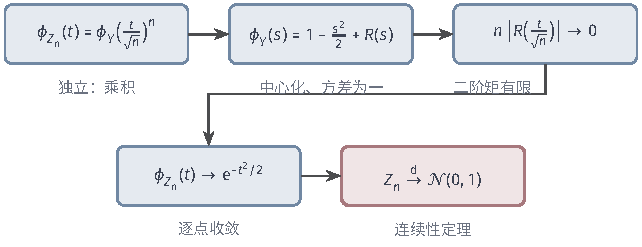
\includegraphics[width=109mm]{figures/07-probability/03-probability-limits/tikz/clt-proof-flow/figure.pdf}
 \caption{中心极限定理的特征函数证明。方框是各步得到的结论，框下灰字是该步所用的条件或工具，红框是要证明的依分布收敛。}
 \label{fig:clt-proof-flow}
\end{BookInlineFigure}

\paragraph{去掉中心化会怎样}
若不减去$\mu$，直接看$S_n/(\sigma\sqrt{n})$，它的特征函数多出因子$\mathrm{e}^{\mathrm{i}t\sqrt{n}\mu/\sigma}$。$\mu\neq0$时这个因子绕单位圆越转越快，对$t\neq0$没有极限，分布的位置以$\sqrt{n}$的速度跑向无穷。中心化就是把这个漂移去掉。

\paragraph{硬币的特征函数}
用硬币核对一遍。把一次结果写成$Y=2X-1$，以各$1/2$的概率取$\pm1$，它已经中心化且方差为一。它的特征函数是
\[
 \phi_Y(s)=\tfrac12\mathrm{e}^{\mathrm{i}s}+\tfrac12\mathrm{e}^{-\mathrm{i}s}=\cos s .
\]
由式~\eqref{eq:clt-product}，$\phi_{Z_n}(t)=\cos(t/\sqrt{n})^{n}$。取$t=1$，$n=1,4,16$时依次为
\[
 \cos1\approx0.5403,\qquad \cos(0.5)^{4}\approx0.5931,\qquad \cos(0.25)^{16}\approx0.6033 ,
\]
极限值是$\mathrm{e}^{-1/2}\approx0.6065$。$n=16$时，近似式$(1-t^2/(2n))^n=(1-1/32)^{16}\approx0.6017$也已接近极限。

证明中的几个量也可以在这里逐一算出。$n=16$、$t=1$时$s=1/4$，单个因子的误差是
\[
 \Bigl\lvert\cos\frac14-\Bigl(1-\frac{1}{32}\Bigr)\Bigr\rvert\approx\lvert0.968912-0.968750\rvert\approx1.62\times10^{-4} ,
\]
乘以$n=16$得到约$2.6\times10^{-3}$。第三步说两个乘积之差不超过这个数，实际的差是
\[
 \lvert0.6033-0.6017\rvert\approx1.6\times10^{-3} .
\]
第一步的上界中$\lvert Y\rvert=1$，它给出
\[
 t^2\,\mathbb{E}\Bigl[\min\Bigl\{\frac{\lvert t\rvert\,\lvert Y\rvert^{3}}{6\sqrt{n}},\ Y^2\Bigr\}\Bigr]=\frac{1}{24}\approx0.042 ,
\]
比实际误差大得多。原因是硬币对称，$\mathbb{E}[Y^3]=0$，$\cos s$的展开中没有三次项，误差从四次项$s^4/24$开始；引理~\ref{lem:clt-exp-remainder}不知道这种对称性，只能按三次估计。证明只需要误差趋于零，不需要它紧。

图~\ref{fig:clt-charfun-convergence}(a)画出整条曲线。$n=1$时$\cos t$在$t=\pm\pi$处等于$-1$，周期地回到$1$，这反映硬币只取格点值；$n$增大时，第一个回到$1$的位置$t=\pi\sqrt{n}$被推向远处，中间部分贴上$\mathrm{e}^{-t^2/2}$。收敛是逐点的，不是在整条实轴上一致的：$t=\pi\sqrt{n}$处总有$\lvert\phi_{Z_n}\rvert=1$。连续性定理只需要逐点收敛。图~\ref{fig:clt-charfun-convergence}(b)是指数等待时间的情形，特征函数取复值，画的是实部，它从一开始就向零衰减，几项以后就与高斯曲线难以区分。

\begin{BookInlineFigure}
 \centering
 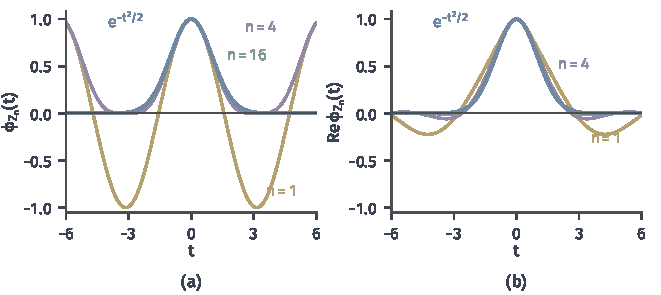
\includegraphics[width=112mm]{figures/07-probability/03-probability-limits/matplotlib/clt-charfun-convergence/figure.pdf}
 \caption{标准化和的特征函数与$\mathrm{e}^{-t^2/2}$（蓝）的比较，$n=1$（黄）、$4$（紫）、$16$（绿；与蓝线几乎重合）。(a)$\pm1$等可能的硬币，$\phi_{Z_n}(t)=\cos(t/\sqrt{n})^{n}$；(b)$\operatorname{Exp}(1)$等待时间，$\phi_{Z_n}(t)=\mathrm{e}^{-\mathrm{i}t\sqrt{n}}(1-\mathrm{i}t/\sqrt{n})^{-n}$的实部。}
 \label{fig:clt-charfun-convergence}
\end{BookInlineFigure}

\subsection{样本平均的正态近似}
\label{sec:clt-sample-mean}

实际使用时，人们关心的是$\bar{X}_n$落在某个区间的概率。把$Z_n\leq x$改写成$\bar{X}_n\leq\mu+x\sigma/\sqrt{n}$，式~\eqref{eq:clt-iid-cdf}就是
\begin{equation}
 \mathbb{P}\Bigl(\bar{X}_n\leq\mu+\frac{x\sigma}{\sqrt{n}}\Bigr)\to\Phi(x),\qquad x\in\mathbb{R} .
 \label{eq:clt-sample-mean}
\end{equation}
人们常把它简写成$\bar{X}_n\approx\mathcal{N}(\mu,\sigma^2/n)$。这个记号的含义是：在$\mu$附近、以$\sigma/\sqrt{n}$为单位量出的阈值上，$\bar{X}_n$的分布函数接近相应的高斯分布函数。

近似的中心是总体均值$\mu$，尺度是$\sigma/\sqrt{n}$，两者都要对。中心取错一个固定量$c$，以$\sigma/\sqrt{n}$为单位就差了$c\sqrt{n}/\sigma$个单位，$n$越大错得越远；尺度用$\sigma/n$或$\sigma$，就回到了第~\ref{sec:clt-scales}节中$a\neq1/2$的情形。

\paragraph{高斯样本：精确}
若$X_i\sim\mathcal{N}(\mu,\sigma^2)$独立，第~\ref{chap:multivariate-distributions}章的线性组合公式给出，对每个$n$，
\[
 \bar{X}_n\sim\mathcal{N}\Bigl(\mu,\frac{\sigma^2}{n}\Bigr),\qquad Z_n\sim\mathcal{N}(0,1) .
\]
这时式~\eqref{eq:clt-sample-mean}左边恒等于$\Phi(x)$，不需要取极限。对一般的样本，式~\eqref{eq:clt-sample-mean}只是$n\to\infty$时的结论，它本身不告诉我们在$n=20$或$n=100$时误差有多大。

\paragraph{二项计数}
设$S\sim\operatorname{Bin}(20,0.3)$，则$np=6$，$np(1-p)=4.2$。精确地，
\[
 \mathbb{P}(S\leq8)\approx0.8867 .
\]
直接套用$\mathcal{N}(6,4.2)$，
\[
 \Phi\Bigl(\frac{8-6}{\sqrt{4.2}}\Bigr)=\Phi(0.976)\approx0.8354 ,
\]
差了约$0.05$。

误差的一个来源是$S$只取整数。$\mathbb{P}(S\leq8)$和$\mathbb{P}(S<9)$是同一个数，阈值在$[8,9)$内任意移动，左边都不变，高斯分布函数却在这一段上从$0.835$升到$0.928$。取中点$8.5$作为阈值，
\[
 \Phi\Bigl(\frac{8.5-6}{\sqrt{4.2}}\Bigr)=\Phi(1.220)\approx0.8887 ,
\]
误差降到$0.002$。这种做法称为\term{连续性修正}（continuity correction）。章首的硬币也一样：$\mathbb{P}(S_{100}\leq55)\approx0.8644$，不修正的近似值是$\Phi(1)\approx0.8413$，修正后是$\Phi(1.1)\approx0.8643$。

图~\ref{fig:clt-binomial-cdf}画出$\operatorname{Bin}(20,0.3)$的分布函数阶梯和两条高斯曲线。不修正的蓝线大致在每级台阶的中点处达到台阶的高度，在整数阈值处偏低；修正后的黄线整体左移半格，在台阶的左端点，也就是整数阈值处，与阶梯的高度相合。连续性修正只是格点分布上的一个经验做法，它不改变极限，也不提供误差保证；有保证的误差界在第~\ref{sec:clt-error}节给出。

\begin{BookInlineFigure}
 \centering
 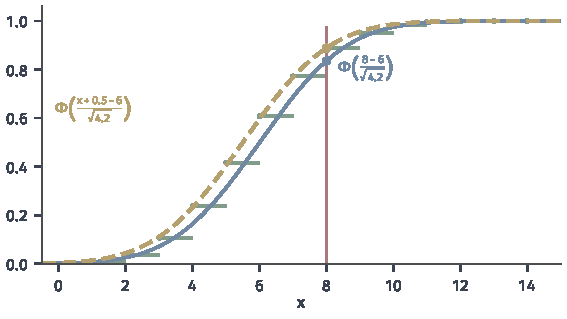
\includegraphics[width=96mm]{figures/07-probability/03-probability-limits/matplotlib/clt-binomial-cdf/figure.pdf}
 \caption{$S\sim\operatorname{Bin}(20,0.3)$的分布函数（绿色阶梯）、高斯近似$\Phi((x-6)/\sqrt{4.2})$（蓝）与连续性修正后的$\Phi((x+0.5-6)/\sqrt{4.2})$（黄色虚线）。红线标出阈值$8$，三点依次为精确值$0.8867$、修正值$0.8887$与未修正值$0.8354$。}
 \label{fig:clt-binomial-cdf}
\end{BookInlineFigure}

\paragraph{需要掷多少次}
正态近似也可以反过来用：给定精度，估计所需的样本量。要使硬币的正面比例与$1/2$相差不超过$0.01$的概率约为$0.95$，由式~\eqref{eq:clt-sample-mean}，需要$0.01$约等于$1.96$个$\sigma/\sqrt{n}$，其中$1.96$是标准高斯分布的$97.5\%$分位数。代入$\sigma=1/2$，
\[
 1.96\cdot\frac{1/2}{\sqrt{n}}=0.01,\qquad n=\Bigl(\frac{1.96\times0.5}{0.01}\Bigr)^2=9604 .
\]

用第~\ref{chap:tail-probabilities}章的Chebyshev不等式也能回答这个问题，而且答案有保证：要使比例偏离$1/2$至少$0.01$的概率不超过$0.05$，只需
\[
 \frac{\sigma^2}{n\cdot0.01^2}=\frac{0.25}{0.0001\,n}\leq0.05,\qquad n\geq50000 .
\]
两个答案相差五倍多。Chebyshev不等式对一切方差为$1/4$的分布都成立，所以保守；正态近似利用了“和接近高斯”这一额外信息，所以省得多，但它只是近似。$n=9604$时这个近似有多准，要等第~\ref{sec:clt-error}节的误差界来回答。

\paragraph{偏斜样本}
指数等待时间没有格点问题，误差来自偏斜。$n=10$时，平均等待时间不超过均值$1$的概率是
\[
 \mathbb{P}(\bar{X}_{10}\leq1)=\mathbb{P}(S_{10}\leq10)\approx0.5421 ,
\]
而式~\eqref{eq:clt-sample-mean}给出$\Phi(0)=0.5$。右偏的分布把中位数拉到均值左边，均值处的分布函数值因此超过$1/2$。图~\ref{fig:clt-gamma-densities}中$n=16$的密度峰仍略偏左，是同一现象。


\section{独立非同分布情形}
\label{sec:clt-non-identical}

一批测量由精度不同的仪器完成，各次误差独立，方差却各不相同；或者每一项的分布本身随总项数变化，像第~\ref{sec:clt-standardization}节的特制硬币。这时没有共同的$\sigma$，标准化只能用总和的标准差。问题变成：各项方差不同，甚至分布随规模改变，什么时候和仍然近似高斯？上一节的特制硬币说明答案不会是“总是”，需要一个条件把“少数几项决定总和”的情形排除掉。

\subsection{三角阵与总方差}
\label{sec:clt-triangular}

各项的分布可以随规模$n$改变，所以把每个规模下的求和项单独列成一行。

\begin{definition}[三角阵]
\label{def:clt-triangular-array}
对每个$n\geq1$，设$k_n$是正整数，$X_{n,1},\dots,X_{n,k_n}$是一组相互独立的随机变量，满足
\begin{equation}
 \mathbb{E}[X_{n,k}]=0,\qquad \sigma_{n,k}^2=\operatorname{Var}(X_{n,k})<\infty .
 \label{eq:clt-array-moments}
\end{equation}
记第$n$行的和与总方差为
\begin{equation}
 S_n=\sum_{k=1}^{k_n}X_{n,k},\qquad s_n^2=\sum_{k=1}^{k_n}\sigma_{n,k}^2 ,
 \label{eq:clt-row-variance}
\end{equation}
并要求$0<s_n^2<\infty$。这样的一族随机变量称为\term{三角阵}（triangular array）。
\end{definition}

名字来自$k_n=n$时的排列方式：第$n$行有$n$项，各行左对齐排成三角形，见图~\ref{fig:clt-triangular-array}。定义只要求同一行内的变量相互独立，不要求不同行之间独立，甚至不要求它们定义在同一个概率空间上。原因是我们只关心每一行的和$S_n$的分布，而$S_n$的分布只由第$n$行的联合分布决定。

\begin{BookInlineFigure}
 \centering
 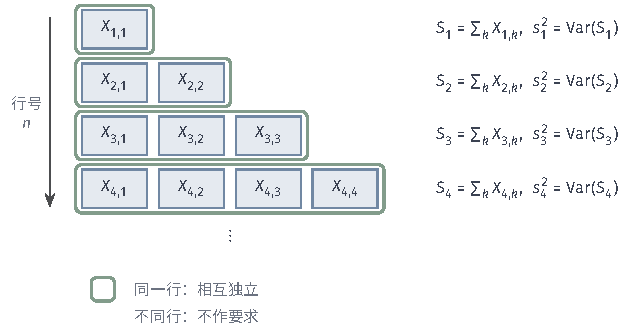
\includegraphics[width=107mm]{figures/07-probability/03-probability-limits/tikz/clt-triangular-array/figure.pdf}
 \caption{三角阵的结构（图中取$k_n=n$）。每一行是一组中心化的求和项，绿框表示行内相互独立；行和$S_n$与总方差$s_n^2$逐行计算，不同行之间不作任何要求。}
 \label{fig:clt-triangular-array}
\end{BookInlineFigure}

由行内独立，$\operatorname{Var}(S_n)=s_n^2$。把各项除以$s_n$，
\[
 \sum_{k=1}^{k_n}\operatorname{Var}\Bigl(\frac{X_{n,k}}{s_n}\Bigr)=\frac{1}{s_n^2}\sum_{k=1}^{k_n}\sigma_{n,k}^2=1 ,
\]
归一化后的各项方差之和为一，$S_n/s_n$均值为零、方差为一。比值$\sigma_{n,k}^2/s_n^2$就是第$k$项在总方差中所占的份额。

\paragraph{独立同分布是特例}
定理~\ref{thm:clt-iid}的情形可以写成三角阵：取$k_n=n$，$X_{n,k}=X_k-\mu$，与$n$无关，则$s_n^2=n\sigma^2$，$S_n/s_n=Z_n$。每一行只是上一行再加一项。三角阵的一般性在于允许各项随$n$整体改变。

\paragraph{三个例子}
本节用下面三个三角阵检验各个条件，它们都满足定义~\ref{def:clt-triangular-array}。
\begin{itemize}
 \item 例A：$X_{n,k}\sim\operatorname{Unif}(-k,k)$，$k=1,\dots,n$。各项有界，方差为$k^2/3$，越往后越大。由$\sum_{k=1}^{n}k^2=n(n+1)(2n+1)/6$，
 \[
  s_n^2=\frac{n(n+1)(2n+1)}{18} .
 \]
 \item 例B：$X_{n,k}\sim\mathcal{N}(0,2^{k})$，$k=1,\dots,n$。方差逐项加倍，$s_n^2=2^{n+1}-2$，最后一项约占总方差的一半。
 \item 例C：$X_{n,k}=B_{n,k}-1/n$，$B_{n,k}\sim\operatorname{Bern}(1/n)$，$k=1,\dots,n$。这是特制硬币的中心化，各项方差都是$\frac1n(1-\frac1n)$，$s_n^2=1-1/n$。
\end{itemize}
例C的行和是$S_n=\operatorname{Bin}(n,1/n)-1$，第~\ref{sec:clt-standardization}节已经看到它的极限不是高斯分布。例B的各项是独立高斯变量，由第~\ref{chap:multivariate-distributions}章，它们的和仍是高斯变量，$S_n\sim\mathcal{N}(0,s_n^2)$，于是对每个$n$都有$S_n/s_n\sim\mathcal{N}(0,1)$。

\subsection{Lindeberg条件}
\label{sec:clt-lindeberg}

例C的毛病在于：总和的波动几乎全部来自“偶尔取到大值”的项。每一项$X_{n,k}$以概率$1/n$取值$1-1/n$，这个值与行的标准差$s_n\approx1$同阶。把方差按取值的大小拆开，例C的方差几乎全部来自那些与$s_n$同阶的取值。要排除这种情形，就要求方差中来自“大值”的部分可以忽略。

\paragraph{截断二阶矩}
固定$\varepsilon>0$，把“大值”理解为绝对值超过$\varepsilon s_n$的取值。每一项的方差拆成两部分，
\[
 \sigma_{n,k}^2=\mathbb{E}\bigl[X_{n,k}^2\mathbf{1}_{\{\lvert X_{n,k}\rvert\leq\varepsilon s_n\}}\bigr]+\mathbb{E}\bigl[X_{n,k}^2\mathbf{1}_{\{\lvert X_{n,k}\rvert>\varepsilon s_n\}}\bigr] .
\]
后一部分是大值贡献的方差。把整行的这部分加起来，再除以总方差，得到大值贡献的份额
\begin{equation}
 L_n(\varepsilon)=\frac{1}{s_n^2}\sum_{k=1}^{k_n}\mathbb{E}\bigl[X_{n,k}^2\mathbf{1}_{\{\lvert X_{n,k}\rvert>\varepsilon s_n\}}\bigr] .
 \label{eq:clt-lindeberg-ratio}
\end{equation}
$L_n(\varepsilon)$在$0$和$1$之间，随$\varepsilon$增大而不增。

\begin{definition}[Lindeberg条件]
\label{def:clt-lindeberg}
称三角阵满足\term{Lindeberg条件}（Lindeberg condition），如果对每个$\varepsilon>0$，
\begin{equation}
 L_n(\varepsilon)\to0\qquad(n\to\infty) .
 \label{eq:clt-lindeberg}
\end{equation}
\end{definition}

条件要求对每个$\varepsilon$都成立，$\varepsilon$越小，被算作大值的范围越宽，要求越严。它说的是：无论把门槛定在总标准差的多小一个比例上，越过门槛的取值所贡献的方差都终将可以忽略。

\paragraph{它推出单项份额趋零}
Lindeberg条件首先保证没有哪一项的方差占总方差的可观份额。对每一项，把方差按$\lvert X_{n,k}\rvert\leq\varepsilon s_n$与否拆开：前一部分不超过$\varepsilon^2s_n^2$，后一部分不超过整行大值贡献之和$s_n^2L_n(\varepsilon)$。于是
\begin{equation}
 \max_{1\leq k\leq k_n}\frac{\sigma_{n,k}^2}{s_n^2}\leq\varepsilon^2+L_n(\varepsilon) .
 \label{eq:clt-max-share}
\end{equation}
令$n\to\infty$，右边的上极限不超过$\varepsilon^2$；$\varepsilon$任意，所以最大份额趋于零。反过来不成立：例C的每一项份额都是$1/n$，趋于零，Lindeberg条件却不成立。单项方差小，不等于大值的贡献小。

\begin{theorem}[Lindeberg中心极限定理]
\label{thm:clt-lindeberg}
设三角阵满足Lindeberg条件~\eqref{eq:clt-lindeberg}。则
\begin{equation}
 \frac{S_n}{s_n}\xrightarrow{\mathrm{d}}\mathcal{N}(0,1) .
 \label{eq:clt-lindeberg-limit}
\end{equation}
\end{theorem}

证明的结构与定理~\ref{thm:clt-iid}相同，仍是比较特征函数的乘积。不同之处在于各因子不再相同，余项要逐项估计后再求和；Lindeberg条件正好控制余项之和。

\begin{proof}
把$X_{n,k}$换成$X_{n,k}/s_n$，可以设$s_n=1$，这时式~\eqref{eq:clt-lindeberg-ratio}中的门槛就是$\varepsilon$。固定$t$和$\varepsilon\in(0,1)$，记$\phi_{n,k}$为$X_{n,k}$的特征函数，并令
\[
 w_{n,k}=1-\frac{t^2\sigma_{n,k}^2}{2} .
\]

第一步，单项误差。在式~\eqref{eq:clt-exp-remainder}中令$x=tX_{n,k}$取期望，与定理~\ref{thm:clt-iid}证明的第一步相同，得到
\[
 \lvert\phi_{n,k}(t)-w_{n,k}\rvert\leq\mathbb{E}\Bigl[\min\Bigl\{\frac{\lvert t\rvert^{3}\lvert X_{n,k}\rvert^{3}}{6},\ t^2X_{n,k}^2\Bigr\}\Bigr] .
\]
在$\{\lvert X_{n,k}\rvert\leq\varepsilon\}$上用三次界，并利用$\lvert X_{n,k}\rvert^3\leq\varepsilon X_{n,k}^2$；在其余部分用二次界。于是
\[
 \lvert\phi_{n,k}(t)-w_{n,k}\rvert\leq\frac{\lvert t\rvert^{3}\varepsilon}{6}\sigma_{n,k}^2+t^2\,\mathbb{E}\bigl[X_{n,k}^2\mathbf{1}_{\{\lvert X_{n,k}\rvert>\varepsilon\}}\bigr] .
\]

第二步，求和。对$k$求和，由$\sum_k\sigma_{n,k}^2=1$与式~\eqref{eq:clt-lindeberg-ratio}，
\[
 \sum_{k=1}^{k_n}\lvert\phi_{n,k}(t)-w_{n,k}\rvert\leq\frac{\lvert t\rvert^{3}\varepsilon}{6}+t^2L_n(\varepsilon) .
\]

第三步，比较乘积。由式~\eqref{eq:clt-max-share}，最大份额趋于零，所以$n$充分大时每个$t^2\sigma_{n,k}^2\leq2$，从而$\lvert w_{n,k}\rvert\leq1$。由行内独立，$\phi_{S_n}(t)=\prod_k\phi_{n,k}(t)$。用引理~\ref{lem:clt-product-difference}，
\[
 \Bigl\lvert\phi_{S_n}(t)-\prod_{k=1}^{k_n}w_{n,k}\Bigr\rvert\leq\frac{\lvert t\rvert^{3}\varepsilon}{6}+t^2L_n(\varepsilon) .
\]
令$n\to\infty$，右边趋于$\lvert t\rvert^3\varepsilon/6$。$\varepsilon$可以任意小，所以左边趋于零。

第四步，乘积的极限。记$a_k=t^2\sigma_{n,k}^2/2\geq0$，则$\sum_ka_k=t^2/2$，而
\[
 \mathrm{e}^{-t^2/2}=\prod_{k=1}^{k_n}\mathrm{e}^{-a_k} .
\]
对$a\geq0$，由带余项的Taylor公式，$\mathrm{e}^{-a}=1-a+\mathrm{e}^{-\xi}a^2/2$，其中$\xi\in(0,a)$，所以$\lvert\mathrm{e}^{-a}-(1-a)\rvert\leq a^2/2$。$\mathrm{e}^{-a_k}$与$w_{n,k}=1-a_k$的模都不超过$1$，再用引理~\ref{lem:clt-product-difference}，
\[
 \Bigl\lvert\prod_{k}w_{n,k}-\mathrm{e}^{-t^2/2}\Bigr\rvert\leq\sum_k\frac{a_k^2}{2}\leq\frac{\max_ka_k}{2}\sum_ka_k=\frac{t^4}{8}\max_k\sigma_{n,k}^2 .
\]
最大份额趋于零，右边趋于零。

第三、四步合起来，$\phi_{S_n}(t)\to\mathrm{e}^{-t^2/2}$对每个$t$成立，由连续性定理得到式~\eqref{eq:clt-lindeberg-limit}。
\end{proof}

证明中Lindeberg条件出现在第三步：小值部分用三次界，贡献至多$\varepsilon$；大值部分只能用二次界，贡献正是$L_n(\varepsilon)$。第四步还需要每项份额都小，这由式~\eqref{eq:clt-max-share}从Lindeberg条件推出。

\paragraph{独立同分布的情形}
对定理~\ref{thm:clt-iid}的三角阵，$Y=(X_1-\mu)/\sigma$，各项同分布，
\[
 L_n(\varepsilon)=\frac{1}{n\sigma^2}\cdot n\,\mathbb{E}\bigl[(X_1-\mu)^2\mathbf{1}_{\{\lvert X_1-\mu\rvert>\varepsilon\sigma\sqrt{n}\}}\bigr]
 =\mathbb{E}\bigl[Y^2\mathbf{1}_{\{\lvert Y\rvert>\varepsilon\sqrt{n}\}}\bigr] .
\]
被积函数被$Y^2$控制，并对每个样本点最终为零，由支配收敛定理，$L_n(\varepsilon)\to0$。所以定理~\ref{thm:clt-iid}是定理~\ref{thm:clt-lindeberg}的特例，二阶矩有限恰好就是独立同分布时的Lindeberg条件。

\paragraph{三个例子的核验}
图~\ref{fig:clt-lindeberg-shares}取$n=20$，$\varepsilon=0.5$，把每一项的方差份额$\sigma_{n,k}^2/s_n^2$画成柱，柱中红色部分是大值的贡献，红色部分之和就是$L_{20}(0.5)$。三个例子的结果分别是
\[
 \text{A}:\ 0.208,\qquad \text{B}:\ 0.749,\qquad \text{C}:\ 0.95 .
\]

\begin{BookInlineFigure}
 \centering
 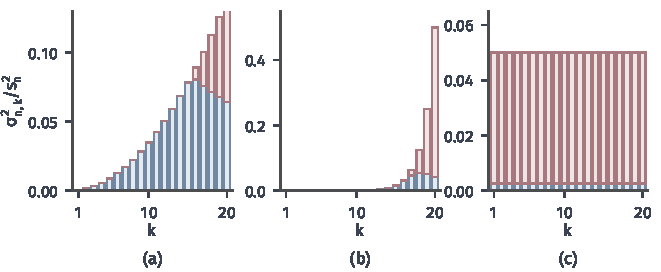
\includegraphics[width=112mm]{figures/07-probability/03-probability-limits/matplotlib/clt-lindeberg-shares/figure.pdf}
 \caption{$n=20$、$\varepsilon=0.5$时各项的方差份额$\sigma_{n,k}^2/s_n^2$。蓝色部分来自$\lvert X_{n,k}\rvert\leq\varepsilon s_n$的取值，红色部分来自$\lvert X_{n,k}\rvert>\varepsilon s_n$的取值，红色之和为$L_{20}(0.5)$。(a)例A，$\operatorname{Unif}(-k,k)$；(b)例B，$\mathcal{N}(0,2^{k})$；(c)例C，中心化的$\operatorname{Bern}(1/20)$。纵轴刻度各不相同。}
 \label{fig:clt-lindeberg-shares}
\end{BookInlineFigure}

例A中$s_{20}^2\approx956.7$，门槛$\varepsilon s_{20}\approx15.5$，只有$k\geq16$的几项可能越过门槛。$\operatorname{Unif}(-k,k)$越过$c<k$的部分贡献
\[
 \mathbb{E}\bigl[X^2\mathbf{1}_{\{\lvert X\rvert>c\}}\bigr]=2\int_c^k\frac{x^2}{2k}\,\mathrm{d}x=\frac{k^3-c^3}{3k} .
\]
代入$c=\varepsilon s_{20}\approx15.465$，$k=16,\dots,20$五项越过门槛的贡献依次约为
\[
 8.28,\quad 23.81,\quad 39.51,\quad 55.44,\quad 71.69 ,
\]
合计约$198.7$，除以$s_{20}^2\approx956.7$得$L_{20}(0.5)\approx0.208$。越往后的项方差越大，越过门槛的部分也越多，图中红色集中在右端。

随着$n$增大，门槛$\varepsilon s_n$按$n^{3/2}$增长，而各项的取值不超过$n$。对$\varepsilon=0.5$，从$n=35$起$\varepsilon s_n\geq n$，没有任何一项能越过门槛，$L_n(0.5)=0$。对任意固定的$\varepsilon>0$同样如此，所以例A满足Lindeberg条件，$S_n/s_n\xrightarrow{\mathrm{d}}\mathcal{N}(0,1)$。

例C中门槛$0.5s_n$小于$0.5$。$n\geq3$时，每一项以概率$1/n$取到的值$1-1/n$越过门槛，另一个取值$-1/n$不越过。所以
\[
 L_n(0.5)=\frac{1}{s_n^2}\cdot n\cdot\frac1n\Bigl(1-\frac1n\Bigr)^{2}=1-\frac1n\to1 .
\]
条件不成立，极限也确实不是高斯分布。

\paragraph{不是必要条件}
例B的$L_n(0.5)$稳定在$0.749$附近，Lindeberg条件不成立，可是$S_n/s_n$对每个$n$都恰好服从$\mathcal{N}(0,1)$。原因是例B的大项本身就是高斯的：最后一项独占一半方差，它的形状直接留在和里，而它碰巧是钟形。所以Lindeberg条件是充分条件，不是中心极限定理的必要条件。

图~\ref{fig:clt-lindeberg-ratio}画出三个例子的$L_n(0.5)$与最大份额随$n$的变化。例A两条曲线都趋于零；例B两条都不趋于零；例C的最大份额$1/n$趋于零，$L_n$却趋于一。

\begin{BookInlineFigure}
 \centering
 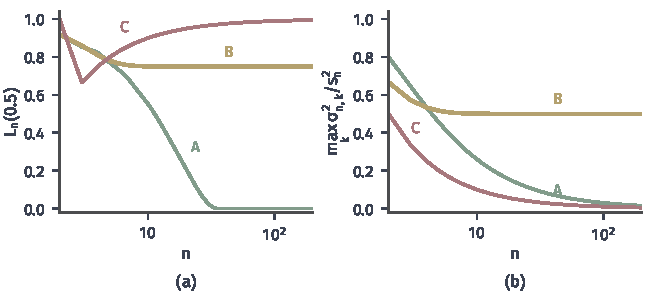
\includegraphics[width=112mm]{figures/07-probability/03-probability-limits/matplotlib/clt-lindeberg-ratio/figure.pdf}
 \caption{三个三角阵的(a)Lindeberg比值$L_n(0.5)$与(b)最大方差份额$\max_k\sigma_{n,k}^2/s_n^2$，$n=2,\dots,200$，横轴为对数刻度。绿为例A，黄为例B，红为例C。}
 \label{fig:clt-lindeberg-ratio}
\end{BookInlineFigure}

例B也说明了缺什么才能反推。若最大份额趋于零，并且$S_n/s_n\xrightarrow{\mathrm{d}}\mathcal{N}(0,1)$，则Lindeberg条件一定成立，这是Feller的逆定理，证明需要更细的特征函数估计，篇幅较长，读者可查阅~\scite{math-kallenberg2021probability}。在“没有一项占优”的前提下，Lindeberg条件就是高斯极限的充要条件；例B不满足这个前提，所以不构成矛盾。

\subsection{Lyapunov条件}
\label{sec:clt-lyapunov}

核验Lindeberg条件要计算截断二阶矩，像例A那样对每一项求越过门槛的部分，往往并不方便。如果各项有略高于二阶的矩，可以用一个更容易计算的量代替它。

\paragraph{用高阶矩压住截断}
在$\{\lvert x\rvert>\varepsilon s_n\}$上，$\lvert x\rvert/(\varepsilon s_n)>1$，于是对任意$\delta>0$，
\[
 x^2\leq x^2\Bigl(\frac{\lvert x\rvert}{\varepsilon s_n}\Bigr)^{\delta}=\frac{\lvert x\rvert^{2+\delta}}{\varepsilon^{\delta}s_n^{\delta}} .
\]
截断二阶矩因此不超过$2+\delta$阶绝对矩除以$\varepsilon^{\delta}s_n^{\delta}$。门槛越高，越过它的取值越大，高阶矩对它们的加权越重，这个不等式正是利用了这一点。

\begin{theorem}[Lyapunov中心极限定理]
\label{thm:clt-lyapunov}
设三角阵的各项具有有限的$2+\delta$阶绝对矩，其中$\delta>0$固定，并且
\begin{equation}
 \Lambda_n(\delta)=\frac{1}{s_n^{2+\delta}}\sum_{k=1}^{k_n}\mathbb{E}\bigl[\lvert X_{n,k}\rvert^{2+\delta}\bigr]\to0 .
 \label{eq:clt-lyapunov}
\end{equation}
则Lindeberg条件成立，从而$S_n/s_n\xrightarrow{\mathrm{d}}\mathcal{N}(0,1)$。
\end{theorem}

条件~\eqref{eq:clt-lyapunov}称为\term{Lyapunov条件}（Lyapunov condition）。

\begin{proof}
对每一项用上面的不等式再取期望，并对$k$求和，
\[
 L_n(\varepsilon)\leq\frac{1}{s_n^2}\sum_{k=1}^{k_n}\frac{\mathbb{E}\bigl[\lvert X_{n,k}\rvert^{2+\delta}\bigr]}{\varepsilon^{\delta}s_n^{\delta}}=\frac{\Lambda_n(\delta)}{\varepsilon^{\delta}} .
\]
对每个固定的$\varepsilon>0$，右边趋于零，这就是Lindeberg条件。再由定理~\ref{thm:clt-lindeberg}得到结论。
\end{proof}

\paragraph{例A的三阶矩}
取$\delta=1$。$\operatorname{Unif}(-k,k)$的三阶绝对矩是
\[
 \mathbb{E}\bigl[\lvert X\rvert^{3}\bigr]=\frac{1}{2k}\int_{-k}^{k}\lvert x\rvert^{3}\,\mathrm{d}x=\frac{k^3}{4} .
\]
由$\sum_{k=1}^{n}k^3=\bigl(n(n+1)/2\bigr)^2$与$s_n^2=n(n+1)(2n+1)/18$，
\[
 \Lambda_n(1)=\frac{n^2(n+1)^2/16}{\bigl(n(n+1)(2n+1)/18\bigr)^{3/2}}\approx\frac{27}{16\sqrt{n}} .
\]
$n=20,100,1000$时，精确值分别约为$0.373$、$0.168$、$0.053$，按$1/\sqrt{n}$趋于零。这里不需要像核验Lindeberg条件那样找出哪些项越过门槛，只要把各项的矩加起来。

\paragraph{有界项}
若存在常数$M$使$\lvert X_{n,k}\rvert\leq M$，并且$s_n\to\infty$，则$\lvert X_{n,k}\rvert^3\leq MX_{n,k}^2$，取期望得
\[
 \mathbb{E}\bigl[\lvert X_{n,k}\rvert^{3}\bigr]\leq M\sigma_{n,k}^2 .
\]
对$k$求和再除以$s_n^3$，
\[
 \Lambda_n(1)\leq\frac{M s_n^2}{s_n^3}=\frac{M}{s_n}\to0 .
\]
所以总方差趋于无穷的一致有界独立项，标准化和总趋于标准高斯分布。例C的各项也有界，但$s_n^2=1-1/n$不趋于无穷，这个推理不适用。

\paragraph{两个条件的比较}
Lyapunov条件多要求了$2+\delta$阶矩，换来的是只需计算未截断的矩之和。它比Lindeberg条件严格地强：设$X_1,X_2,\dots$独立同分布，方差有限，但对每个$\delta>0$都有$\mathbb{E}[\lvert X_1\rvert^{2+\delta}]=\infty$，例如密度在$\lvert x\rvert>\mathrm{e}$上与$1/(\lvert x\rvert^3\ln^2\lvert x\rvert)$成正比的对称分布。这时Lyapunov条件无从谈起，而独立同分布时Lindeberg条件总成立，中心极限定理照样成立。图~\ref{fig:clt-condition-map}汇总了本节的几个条件与结论之间的推出关系。

\begin{BookInlineFigure}
 \centering
 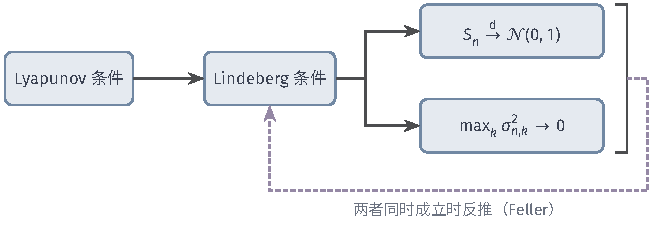
\includegraphics[width=111mm]{figures/07-probability/03-probability-limits/tikz/clt-condition-map/figure.pdf}
 \caption{三角阵各条件与结论的关系（行内独立、中心化、$s_n=1$）。实线箭头表示推出；紫色虚线表示Feller逆定理：高斯极限与最大份额趋零同时成立时，可以反推Lindeberg条件。单有高斯极限推不出Lindeberg条件，例B即是。}
 \label{fig:clt-condition-map}
\end{BookInlineFigure}

这些条件都只是充分条件，或者在附加前提下才是充要条件。把它们当作中心极限定理的必要条件，就会像例B那样误判；反过来，看到“每项方差都很小”就断言高斯极限，又会在例C上出错。


\section{多元中心极限定理}
\label{sec:clt-multivariate}

掷$n$次骰子，记下六个面各出现了多少次；或者同时测量一批零件的长度和重量。这时每次观测是一个向量，平均也是向量。各分量的平均分别近似高斯还不够，我们还想知道它们的偏差怎样联合分布：长度偏大时重量是否也偏大，六个频率之和恒为一这一约束又怎样体现在极限里。

设$\bm{X}_1,\bm{X}_2,\dots$是$\mathbb{R}^{d}$中独立同分布的随机向量，维数$d$固定，$\mathbb{E}[\lVert\bm{X}_1\rVert_2^2]<\infty$。记均值向量为$\bm{\mu}$，协方差矩阵为$\bm{\Sigma}$（粗体大写表示$d\times d$矩阵），样本平均为
\[
 \bar{\bm{X}}_n=\frac1n\sum_{i=1}^{n}\bm{X}_i .
\]
要研究的对象是$\sqrt{n}(\bar{\bm{X}}_n-\bm{\mu})$。这里不除以标准差：向量没有单一的标准差，$\bm{\Sigma}$还可能不可逆。极限中会直接出现$\bm{\Sigma}$本身。

\paragraph{两枚硬币的例子}
设$\xi,\eta$独立，各以$1/2$的概率取$\pm1$，令$\bm{X}=(\xi,\ \xi+\eta)^{\top}$。两个分量共享$\xi$，所以正相关。直接计算，$\bm{\mu}=\bm{0}$，
\[
 \operatorname{Var}(\xi)=1,\qquad \operatorname{Var}(\xi+\eta)=2,\qquad \operatorname{Cov}(\xi,\xi+\eta)=\operatorname{Var}(\xi)=1 ,
\]
即
\[
 \bm{\Sigma}=\begin{bmatrix}1&1\\1&2\end{bmatrix} .
\]
本节还用一个退化的对照：$\bm{X}=(\xi,\ 2\xi)^{\top}$，协方差矩阵的各元为$1,2,2,4$，行列式为零。

\subsection{方向投影}
\label{sec:clt-projection}

向量的分布不容易直接处理，可以先把它投到各个方向上，变成标量问题。固定$\bm{a}\in\mathbb{R}^{d}$，投影$\bm{a}^{\top}\bm{X}_i$是独立同分布的实随机变量。由第~\ref{chap:random-vectors}章的均值与协方差的线性规则，
\[
 \mathbb{E}[\bm{a}^{\top}\bm{X}_i]=\bm{a}^{\top}\bm{\mu},\qquad \operatorname{Var}(\bm{a}^{\top}\bm{X}_i)=\bm{a}^{\top}\bm{\Sigma}\bm{a} .
\]
投影与平均可以交换，$\bm{a}^{\top}\sqrt{n}(\bar{\bm{X}}_n-\bm{\mu})$正是投影序列的$\sqrt{n}$倍平均偏差。按$\bm{a}^{\top}\bm{\Sigma}\bm{a}$是否为零分两种情形。

\paragraph{正方差方向}
若$\bm{a}^{\top}\bm{\Sigma}\bm{a}>0$，投影序列满足定理~\ref{thm:clt-iid}的全部条件，所以
\[
 \frac{\sqrt{n}\,\bm{a}^{\top}(\bar{\bm{X}}_n-\bm{\mu})}{\sqrt{\bm{a}^{\top}\bm{\Sigma}\bm{a}}}\xrightarrow{\mathrm{d}}\mathcal{N}(0,1) .
\]
记左边为$W_n$，再乘回常数$c=\sqrt{\bm{a}^{\top}\bm{\Sigma}\bm{a}}>0$。对每个$x$，
\[
 \mathbb{P}(cW_n\leq x)=\mathbb{P}\Bigl(W_n\leq\frac{x}{c}\Bigr)\to\Phi\Bigl(\frac{x}{c}\Bigr) ,
\]
右边是$\mathcal{N}(0,c^2)$的分布函数。于是
\begin{equation}
 \sqrt{n}\,\bm{a}^{\top}(\bar{\bm{X}}_n-\bm{\mu})\xrightarrow{\mathrm{d}}\mathcal{N}(0,\bm{a}^{\top}\bm{\Sigma}\bm{a}) .
 \label{eq:clt-projection}
\end{equation}

\paragraph{零方差方向}
若$\bm{a}^{\top}\bm{\Sigma}\bm{a}=0$，标准化要除以零，不能套用。这时$\bm{a}^{\top}(\bm{X}_i-\bm{\mu})$均值为零、方差为零，几乎必然等于零。于是对每个$n$，
\[
 \sqrt{n}\,\bm{a}^{\top}(\bar{\bm{X}}_n-\bm{\mu})=\frac{1}{\sqrt{n}}\sum_{i=1}^{n}\bm{a}^{\top}(\bm{X}_i-\bm{\mu})=0\quad\text{几乎必然} .
\]
它的分布恒为$0$处的单点分布，当然依分布收敛到这个单点分布。按第~\ref{sec:clt-standardization}节的约定，单点分布就是$\mathcal{N}(0,0)$，所以式~\eqref{eq:clt-projection}在零方差方向也成立。

\paragraph{两枚硬币的投影}
对$\bm{X}=(\xi,\ \xi+\eta)^{\top}$，三个方向上的极限方差分别是
\[
 \bm{a}=(1,0)^{\top}:\ 1,\qquad \bm{a}=(0,1)^{\top}:\ 2,\qquad \bm{a}=\tfrac{1}{\sqrt2}(1,-1)^{\top}:\ \tfrac12(1-2+2)=\tfrac12 .
\]
最后一个方向是两分量之差，$\xi-(\xi+\eta)=-\eta$，方差本来就是$1$，除以$(\sqrt2)^2$后为$1/2$。图~\ref{fig:clt-projections}用$n=100$、$1500$次重复模拟检验这三个结论，三个直方图的样本方差分别为$0.98$、$1.99$、$0.47$。

\begin{BookInlineFigure}
 \centering
 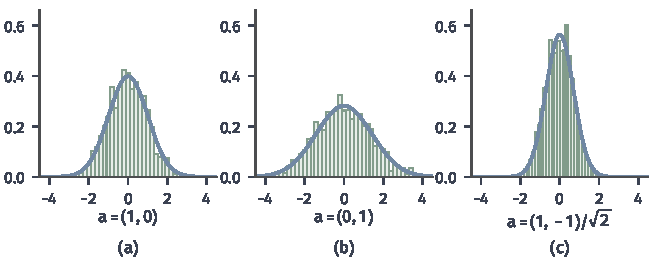
\includegraphics[width=112mm]{figures/07-probability/03-probability-limits/matplotlib/clt-projections/figure.pdf}
 \caption{$\bm{X}=(\xi,\xi+\eta)^{\top}$、$n=100$时$\bm{a}^{\top}\sqrt{n}\,\bar{\bm{X}}_n$的直方图（浅绿，$1500$次重复，种子$3$，每个格点一个柱）与$\mathcal{N}(0,\bm{a}^{\top}\bm{\Sigma}\bm{a})$的密度（蓝）。(a)$\bm{a}=(1,0)^{\top}$，方差$1$；(b)$\bm{a}=(0,1)^{\top}$，方差$2$；(c)$\bm{a}=(1,-1)^{\top}/\sqrt2$，方差$1/2$。}
 \label{fig:clt-projections}
\end{BookInlineFigure}

对退化的$\bm{X}=(\xi,\ 2\xi)^{\top}$，方向$\bm{a}=(2,-1)^{\top}$给出$\bm{a}^{\top}\bm{X}=2\xi-2\xi=0$，这是零方差方向；与它垂直的方向$(1,2)^{\top}/\sqrt5$上，投影是$\sqrt5\,\xi$，方差为$5$。

\subsection{联合高斯极限}
\label{sec:clt-joint}

每个方向上的极限都是高斯的，方差由同一个矩阵$\bm{\Sigma}$按$\bm{a}^{\top}\bm{\Sigma}\bm{a}$给出。第~\ref{chap:multivariate-distributions}章说明，若$\bm{W}\sim\mathcal{N}(\bm{0},\bm{\Sigma})$，则对每个$\bm{a}$，
\begin{equation}
 \bm{a}^{\top}\bm{W}\sim\mathcal{N}(0,\bm{a}^{\top}\bm{\Sigma}\bm{a}) .
 \label{eq:clt-gauss-projection}
\end{equation}
所以各方向的极限恰好是同一个高斯向量$\bm{W}$的各个投影。Cramér--Wold判据说，在固定维数中，所有方向的投影依分布收敛到同一个向量的投影，就足以推出向量本身依分布收敛。

\begin{theorem}[多元中心极限定理]
\label{thm:clt-multivariate}
设$\bm{X}_1,\bm{X}_2,\dots$是$\mathbb{R}^{d}$中独立同分布的随机向量，$\mathbb{E}[\lVert\bm{X}_1\rVert_2^2]<\infty$，均值为$\bm{\mu}$，协方差矩阵为$\bm{\Sigma}$。则
\begin{equation}
 \sqrt{n}\,(\bar{\bm{X}}_n-\bm{\mu})\xrightarrow{\mathrm{d}}\mathcal{N}(\bm{0},\bm{\Sigma}) .
 \label{eq:clt-multivariate}
\end{equation}
\end{theorem}

这个结论称为\term{多元中心极限定理}（multivariate central limit theorem）。

\begin{proof}
设$\bm{W}\sim\mathcal{N}(\bm{0},\bm{\Sigma})$。对每个$\bm{a}\in\mathbb{R}^{d}$，由式~\eqref{eq:clt-projection}，投影$\bm{a}^{\top}\sqrt{n}(\bar{\bm{X}}_n-\bm{\mu})$依分布收敛到$\mathcal{N}(0,\bm{a}^{\top}\bm{\Sigma}\bm{a})$，正方差与零方差方向都包括在内。由式~\eqref{eq:clt-gauss-projection}，这个极限就是$\bm{a}^{\top}\bm{W}$的分布。由Cramér--Wold判据，$\sqrt{n}(\bar{\bm{X}}_n-\bm{\mu})\xrightarrow{\mathrm{d}}\bm{W}$。
\end{proof}

\paragraph{为什么要看所有方向}
只看坐标方向，得到的是每个分量各自的极限，即边缘分布的收敛。第~\ref{chap:weak-convergence-of-distributions}章说明，边缘收敛不能确定分量之间的配对方式。两枚硬币的例子里，两个分量的极限分别是$\mathcal{N}(0,1)$与$\mathcal{N}(0,2)$；它们是相互独立，还是相关系数为$1/\sqrt2$，只有斜方向（例如图~\ref{fig:clt-projections}(c)）的方差能分辨：独立时差的方差应是$\frac12(1+2)=\frac32$，实际是$\frac12$。定理的证明用到了全部方向，所以得到的是联合极限，相关结构由$\bm{\Sigma}$的非对角元保留下来。

图~\ref{fig:clt-bivariate-scatter}(a)把同一批模拟的点$\sqrt{n}\,\bar{\bm{X}}_n$画在平面上，点云沿主对角方向拉长。$\mathcal{N}(\bm{0},\bm{\Sigma})$在马氏距离$1$与$2$以内的概率是$1-\mathrm{e}^{-1/2}\approx0.393$与$1-\mathrm{e}^{-2}\approx0.865$，模拟点落在这两个椭圆内（含边界）的比例是$0.398$与$0.885$，边界上的格点使后者略偏大。点排成格子，因为$n=100$时每个分量只取间距为$0.2$的格点值；依分布收敛并不要求有限$n$的分布有密度。

\begin{BookInlineFigure}
 \centering
 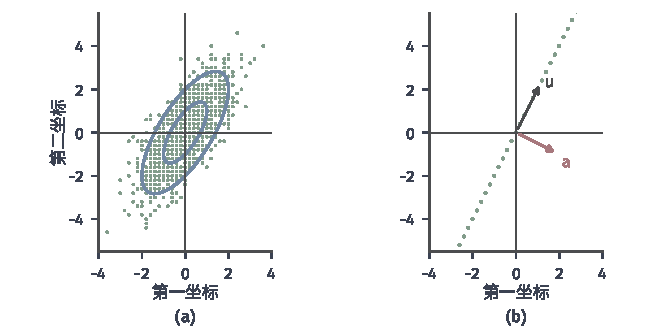
\includegraphics[width=112mm]{figures/07-probability/03-probability-limits/matplotlib/clt-bivariate-scatter/figure.pdf}
 \caption{$n=100$时$\sqrt{n}\,\bar{\bm{X}}_n$的$1500$个模拟点（绿，种子$3$）。(a)$\bm{X}=(\xi,\xi+\eta)^{\top}$，蓝色椭圆是$\mathcal{N}(\bm{0},\bm{\Sigma})$在马氏距离$1$与$2$处的等高线；(b)$\bm{X}=(\xi,2\xi)^{\top}$，点全部落在直线$y=2x$上，红色箭头$\bm{a}$是零方差方向$(2,-1)^{\top}/\sqrt5$，灰色箭头$\bm{u}$是直线方向$(1,2)^{\top}/\sqrt5$。}
 \label{fig:clt-bivariate-scatter}
\end{BookInlineFigure}

\paragraph{奇异的协方差矩阵}
定理不要求$\bm{\Sigma}$可逆。退化例子中$\bm{\Sigma}$的秩为一，极限$\mathcal{N}(\bm{0},\bm{\Sigma})$是第~\ref{chap:multivariate-distributions}章的退化高斯分布，全部质量在直线$\{t(1,2)^{\top}:t\in\mathbb{R}\}$上，在平面上没有密度。图~\ref{fig:clt-bivariate-scatter}(b)中有限$n$的点也都在这条直线上。若要写出标准化的形式$\bm{\Sigma}^{-1/2}\sqrt{n}(\bar{\bm{X}}_n-\bm{\mu})$，就必须假设$\bm{\Sigma}$可逆；式~\eqref{eq:clt-multivariate}的写法避开了这个假设。

\paragraph{骰子的频率}
掷一枚均匀骰子$n$次，令$\bm{X}_i\in\mathbb{R}^{6}$是第$i$次结果的示性向量：出现第$j$面时第$j$个分量为$1$，其余为$0$。$\bar{\bm{X}}_n$就是六个面的频率向量，$n\bar{\bm{X}}_n\sim\operatorname{Mult}(n,\bm{p})$，$\bm{p}=\frac16\bm{1}$。由$X_{i,j}X_{i,k}=0$（$j\neq k$）与$X_{i,j}^2=X_{i,j}$，
\[
 \bm{\Sigma}=\operatorname{diag}(\bm{p})-\bm{p}\bm{p}^{\top},\qquad \Sigma_{j,j}=\frac16-\frac1{36}=\frac{5}{36},\qquad \Sigma_{j,k}=-\frac{1}{36}\ (j\neq k) .
\]
由定理~\ref{thm:clt-multivariate}，$\sqrt{n}(\bar{\bm{X}}_n-\bm{p})\xrightarrow{\mathrm{d}}\mathcal{N}(\bm{0},\bm{\Sigma})$。频率之和恒为一，所以$\bm{1}^{\top}(\bm{X}_i-\bm{p})=0$，$\bm{1}$是零方差方向，$\bm{\Sigma}\bm{1}=\bm{0}$。极限分布集中在“六个偏差之和为零”的五维子空间上，各频率偏差之间是负相关：一个面出现得多，其余的面就只能少。

\paragraph{维数固定}
定理中的$d$在$n\to\infty$时保持不变。它不说明维数随样本量一同增长时会怎样，也不涉及部分和作为$n$的函数、整条随机路径的极限形状；后者需要在函数空间中讨论收敛，超出了有限维概率极限的范围。


\section{正态近似误差}
\label{sec:clt-error}

中心极限定理是$n\to\infty$时的结论，它保证误差趋于零，却不告诉我们$n=100$时误差是$0.04$还是$0.4$。前面的例子已经给出一些具体数字：$\operatorname{Bin}(20,0.3)$在阈值$8$处差了$0.05$，十个指数等待时间的平均在均值处差了$0.042$。本节先确定比较的是哪一种误差，再在多一阶矩的条件下给出对所有阈值同时成立的上界。

\paragraph{比较什么}
设$F_n$是$Z_n$的分布函数。最常用的比较对象是两条分布函数之间的最大竖直距离
\begin{equation}
 D_n=\sup_{x\in\mathbb{R}}\bigl\lvert F_n(x)-\Phi(x)\bigr\rvert .
 \label{eq:clt-kolmogorov}
\end{equation}
它控制所有形如$\{Z_n\leq x\}$的事件，从而控制所有区间事件：$\mathbb{P}(a<Z_n\leq b)$与$\Phi(b)-\Phi(a)$之差不超过$2D_n$。由式~\eqref{eq:clt-iid-cdf}与$\Phi$的连续性，可以证明$D_n\to0$，但定理本身不给出速度。怎样利用这样的近似构造区间并评价其可靠性，属于统计推断的问题，可参考\BookChapterRef{chap:parametric-statistical-inference}{卷八第1章“参数化统计推断”}；这里只研究概率误差本身。

\subsection{Berry--Esseen界}
\label{sec:clt-berry-esseen}

定理~\ref{thm:clt-iid}的证明里，单个因子的误差用了二次界，因为只知道二阶矩。如果三阶绝对矩有限，就可以用三次界：每个因子的误差约为$\lvert t\rvert^3\mathbb{E}[\lvert Y\rvert^3]/(6n^{3/2})$，$n$个因子累计为$\lvert t\rvert^3\mathbb{E}[\lvert Y\rvert^3]/(6\sqrt{n})$。特征函数之差按$1/\sqrt{n}$缩小，分布函数之差也应当如此。

\begin{theorem}[Berry--Esseen界]
\label{thm:clt-berry-esseen}
设$X_1,X_2,\dots$独立同分布，方差$\sigma^2>0$，三阶绝对中心矩$\rho=\mathbb{E}[\lvert X_1-\mu\rvert^{3}]<\infty$。则存在与分布无关的常数$C$，使对每个$n\geq1$，
\begin{equation}
 \sup_{x\in\mathbb{R}}\bigl\lvert\mathbb{P}(Z_n\leq x)-\Phi(x)\bigr\rvert\leq\frac{C\rho}{\sigma^{3}\sqrt{n}} .
 \label{eq:clt-berry-esseen}
\end{equation}
\end{theorem}

这个上界称为\term{Berry--Esseen界}（Berry-Esseen bound）。目前已知可以取$C=0.4748$。证明的关键是一个光滑化不等式：把分布函数之差用特征函数之差在原点附近的积分来控制，再代入上面的三阶估计。这一不等式的推导与常数的优化都较长，读者可查阅~\scite{math-kallenberg2021probability}。

\paragraph{界的含义}
式~\eqref{eq:clt-berry-esseen}有三个特点。它对所有阈值$x$同时成立，所以是一致的；它控制的是概率之差，是绝对误差；它以$1/\sqrt{n}$的速度缩小，样本量变成四倍，误差界减半。分布的影响全部集中在比值$\rho/\sigma^3$上，这是标准化变量$Y$的三阶绝对矩$\mathbb{E}[\lvert Y\rvert^3]$。

这个比值至少是$1$。函数$u\mapsto u^{3/2}$在$[0,\infty)$上是凸函数，对非负变量$Y^2$用Jensen不等式，
\[
 \mathbb{E}\bigl[\lvert Y\rvert^{3}\bigr]=\mathbb{E}\bigl[(Y^2)^{3/2}\bigr]\geq\bigl(\mathbb{E}[Y^2]\bigr)^{3/2}=1 .
\]
等号对以等概率取$\pm1$的$Y$成立。比值越大，说明单项的取值越偏离“正负各一个标准差”，界越松。

\paragraph{三个分布的比值}
对$X\sim\operatorname{Bern}(p)$，$\lvert X-p\rvert$以概率$p$取$1-p$，以概率$1-p$取$p$，记$q=1-p$，
\[
 \rho=pq^3+qp^3=pq(p^2+q^2),\qquad \frac{\rho}{\sigma^3}=\frac{p^2+q^2}{\sqrt{pq}} .
\]
$p=1/2$时比值为$1$，$p=1/10$时为$0.82/0.3\approx2.733$。对$X\sim\operatorname{Exp}(1)$，$\sigma=1$，把积分在$x=1$处分开，
\[
 \int_1^{\infty}(x-1)^3\mathrm{e}^{-x}\,\mathrm{d}x=\frac{6}{\mathrm{e}},\qquad \int_0^1(1-x)^3\mathrm{e}^{-x}\,\mathrm{d}x=\frac{6}{\mathrm{e}}-2 ,
\]
前一个积分换元$u=x-1$后是$\mathrm{e}^{-1}\int_0^\infty u^3\mathrm{e}^{-u}\,\mathrm{d}u$，后一个由三次分部积分得到。合起来$\rho=12/\mathrm{e}-2\approx2.415$。

表~\ref{tab:clt-berry-esseen}比较$n=100$时的上界与精确的最大误差。最大误差由精确分布在所有跳点两侧逐一比较得到；指数情形用$\operatorname{Gamma}(n,1)$的分布函数在细网格上计算。

\begin{BookInlineTable}
 \centering
 \caption{$n=100$时Berry--Esseen上界（$C=0.4748$）与精确最大误差$D_{100}$的比较。}
 \label{tab:clt-berry-esseen}
 \begin{tabular}{lccc}
 \toprule
 单项分布 & $\rho/\sigma^3$ & 上界$C\rho/(\sigma^3\sqrt{100})$ & 精确$D_{100}$ \\
 \midrule
 $\operatorname{Bern}(1/2)$ & $1$ & $0.0475$ & $0.0398$ \\
 $\operatorname{Bern}(1/10)$ & $2.733$ & $0.130$ & $0.0832$ \\
 $\operatorname{Exp}(1)$ & $2.415$ & $0.115$ & $0.0133$ \\
 \bottomrule
 \end{tabular}
\end{BookInlineTable}

回到第~\ref{sec:clt-sample-mean}节掷$9604$次硬币的问题。比值为$1$，每个分布函数值的误差不超过$0.4748/\sqrt{9604}\approx0.0048$，区间概率是两个分布函数值之差，误差不超过$0.0097$。所以那里的“约为$0.95$”可以确切地写成“在$0.94$与$0.96$之间”。

表中硬币的上界只比实际误差大约五分之一，指数等待时间的上界却大了八倍多。图~\ref{fig:clt-berry-esseen-rate}在双对数坐标中画出$n$从$1$到$1000$的情形，所有误差曲线都以斜率$-1/2$下降，与上界平行，各自始终在自己的上界之下。

\begin{BookInlineFigure}
 \centering
 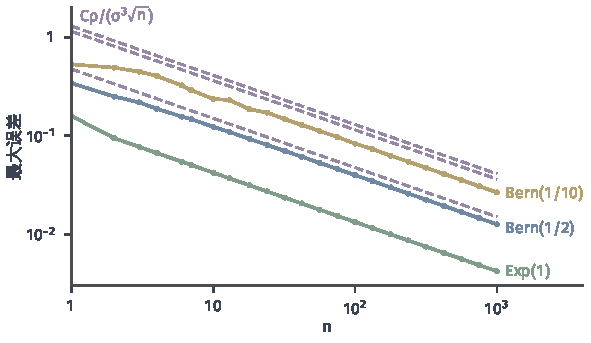
\includegraphics[width=100mm]{figures/07-probability/03-probability-limits/matplotlib/clt-berry-esseen-rate/figure.pdf}
 \caption{标准化和与$\mathcal{N}(0,1)$的精确最大误差$D_n$随$n$的变化，双对数坐标。蓝为$\operatorname{Bern}(1/2)$，黄为$\operatorname{Bern}(1/10)$，绿为$\operatorname{Exp}(1)$。紫色虚线是对应的Berry--Esseen上界$0.4748\rho/(\sigma^3\sqrt{n})$，自上而下依次属于$\operatorname{Bern}(1/10)$、$\operatorname{Exp}(1)$与$\operatorname{Bern}(1/2)$。}
 \label{fig:clt-berry-esseen-rate}
\end{BookInlineFigure}

\paragraph{速度不能更快}
$1/\sqrt{n}$的速度一般不能改进，硬币就是例子。$n$为偶数时，$Z_n$在$0$处有一个原子，质量是$\mathbb{P}(S_n=n/2)$，分布函数在那里跳起这么高，而$\Phi$是连续的。在跳点处，$F_n$的左极限与右值相差这个跳跃，它们与同一个数$\Phi(0)$的距离至少有一个不小于跳跃的一半。所以
\[
 D_n\geq\frac12\,\mathbb{P}\Bigl(S_n=\frac n2\Bigr)=\frac12\binom{n}{n/2}2^{-n} .
\]
$n=100$时右边是$\frac12\times0.0796=0.0398$，正好是表~\ref{tab:clt-berry-esseen}中的精确值。由Stirling公式，$\binom{n}{n/2}2^{-n}\approx\sqrt{2/(\pi n)}$，于是$D_n$至少约为$1/\sqrt{2\pi n}\approx0.399/\sqrt{n}$。这也说明常数$C$不能小于约$0.399$。

\paragraph{误差出现在哪里}
最大误差只是一个数，图~\ref{fig:clt-error-profile}画出带符号的误差$F_n(x)-\Phi(x)$随阈值的变化。指数等待时间的误差是一条光滑的波形，在中心附近为正、两侧为负，这是右偏造成的：均值处的分布函数值$0.542$超过$1/2$。硬币的误差是锯齿形，每过一个格点跳一次，幅度在中心最大；这一误差来自格点结构，任何光滑的近似都无法消除，连续性修正只是把阈值放到台阶中间以减小它。

\begin{BookInlineFigure}
 \centering
 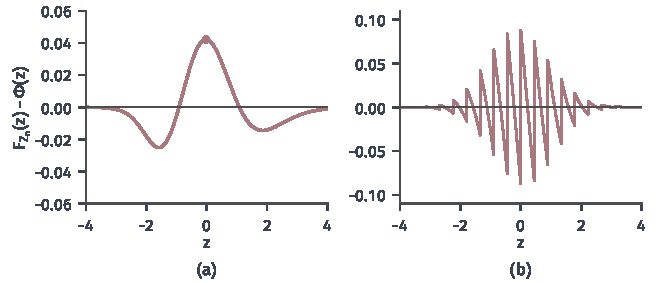
\includegraphics[width=112mm]{figures/07-probability/03-probability-limits/matplotlib/clt-error-profile/figure.pdf}
 \caption{带符号的误差$F_{Z_n}(z)-\Phi(z)$。(a)$\operatorname{Exp}(1)$，$n=10$，红点为最大误差$0.042$，位于$z\approx0$；(b)$\operatorname{Bern}(1/2)$，$n=20$，误差在每个格点处跳跃，最大约$0.088$。}
 \label{fig:clt-error-profile}
\end{BookInlineFigure}

\paragraph{非同分布的情形}
三角阵也有类似的界：若各项三阶绝对矩有限，$S_n/s_n$与$\mathcal{N}(0,1)$的分布函数最大距离不超过一个通用常数乘以
\[
 \frac{1}{s_n^3}\sum_{k=1}^{k_n}\mathbb{E}\bigl[\lvert X_{n,k}\rvert^{3}\bigr] ,
\]
这正是第~\ref{sec:clt-lyapunov}节$\delta=1$时的Lyapunov比值$\Lambda_n(1)$。Lyapunov条件因此不只保证收敛，在$\delta=1$时还直接给出了误差的量级。例A中$\Lambda_n(1)\approx27/(16\sqrt{n})$，误差也按$1/\sqrt{n}$缩小。

\subsection{近似的适用范围}
\label{sec:clt-applicability}

“正态近似可用”这句话要说清楚用于什么精度。表~\ref{tab:clt-accuracy}列出三种不同的要求。前两种已经讨论过；第三种在计算罕见事件的概率时常常遇到，Berry--Esseen界对它几乎没有帮助。

\begin{BookInlineTable}
 \centering
 \caption{正态近似的三种精度要求。}
 \label{tab:clt-accuracy}
 \begin{tabular}{lll}
 \toprule
 精度要求 & 含义 & 本章的依据 \\
 \midrule
 渐近收敛 & 误差随$n$趋于零 & 二阶矩或Lindeberg条件 \\
 一致绝对误差 & 给定$n$时的误差上界 & 三阶矩，Berry--Esseen界 \\
 尾概率相对误差 & 近似值与真值之比 & 本章没有给出 \\
 \bottomrule
 \end{tabular}
\end{BookInlineTable}

\paragraph{小尾概率}
设$p_n(z)=\mathbb{P}(Z_n\geq z)$。由式~\eqref{eq:clt-berry-esseen}，取左极限后同样有
\[
 \bigl\lvert p_n(z)-(1-\Phi(z))\bigr\rvert\leq\frac{C\rho}{\sigma^3\sqrt{n}} ,
\]
右边与$z$无关。当$z$较大时，$1-\Phi(z)$本身可能是$10^{-4}$甚至更小，而右边是$0.1$量级，这个界不能说明近似值有一位有效数字是对的。

十个指数等待时间的精确右尾与高斯近似是
\[
 \begin{aligned}
 z=2:&\quad 0.0369 &&\text{对}\quad 0.0228,\\
 z=3:&\quad 0.00672 &&\text{对}\quad 0.00135,\\
 z=4:&\quad 1.01\times10^{-3} &&\text{对}\quad 3.17\times10^{-5},\\
 z=5:&\quad 1.29\times10^{-4} &&\text{对}\quad 2.87\times10^{-7} .
 \end{aligned}
\]
比值依次约为$1.6$、$5.0$、$32$、$450$。绝对误差都不超过$0.015$，与Berry--Esseen界并不矛盾；相对误差却越来越大。左尾的情形更极端：$S_{10}>0$，所以$Z_{10}>-\sqrt{10}$，$\mathbb{P}(Z_{10}\leq-\sqrt{10})=0$，而高斯近似给出$\Phi(-\sqrt{10})\approx7.8\times10^{-4}$。

图~\ref{fig:clt-relative-tail}在对数纵轴上画出两侧的尾部。右偏的分布右尾比高斯厚，左尾比高斯薄而且在有限处截断。对数坐标暴露出来的这些差别，在普通坐标中都挤在零附近，看不出来。

\begin{BookInlineFigure}
 \centering
 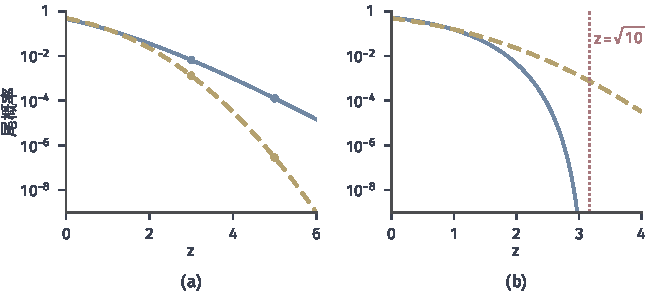
\includegraphics[width=112mm]{figures/07-probability/03-probability-limits/matplotlib/clt-relative-tail/figure.pdf}
 \caption{$n=10$个$\operatorname{Exp}(1)$之和标准化后的尾概率，纵轴为对数刻度。蓝线为精确值，黄色虚线为高斯近似。(a)右尾$\mathbb{P}(Z_{10}\geq z)$与$1-\Phi(z)$，圆点标出$z=3,5$；(b)左尾$\mathbb{P}(Z_{10}\leq-z)$与$\Phi(-z)$，精确左尾在$z=\sqrt{10}$（红色点线）处降为零。}
 \label{fig:clt-relative-tail}
\end{BookInlineFigure}

中心极限定理描述的是距中心几个标准差以内的“典型”波动；离中心越远，概率越依赖单项分布的尾部形状，而不仅是均值和方差。估计罕见事件的概率，应当直接计算精确分布，或使用第~\ref{chap:tail-probabilities}章基于指数矩的上界，它们的误差是按尾概率本身的大小来衡量的。

\paragraph{三阶矩无穷的情形}
Berry--Esseen界需要三阶绝对矩，中心极限定理只需要二阶矩，两者之间有一段空隙。取第~\ref{chap:tail-probabilities}章参数为$3$的Pareto分布，配上等概率的正负号，得到密度
\[
 f(x)=\frac32\lvert x\rvert^{-4},\qquad \lvert x\rvert\geq1 .
\]
它关于原点对称，均值为零。二阶矩与三阶绝对矩分别是
\[
 \mathbb{E}[X^2]=2\int_1^{\infty}x^2\cdot\frac32x^{-4}\,\mathrm{d}x=3,\qquad
 \mathbb{E}\bigl[\lvert X\rvert^3\bigr]=3\int_1^{\infty}x^{-1}\,\mathrm{d}x=\infty .
\]

方差有限，定理~\ref{thm:clt-iid}适用，$S_n/\sqrt{3n}\xrightarrow{\mathrm{d}}\mathcal{N}(0,1)$。图~\ref{fig:clt-pareto-third}的模拟也显示出钟形。可是$\rho=\infty$，式~\eqref{eq:clt-berry-esseen}的右边是无穷，不提供任何信息。收敛的速度需要另作分析：模拟中$\mathbb{P}(\lvert Z_n\rvert\leq0.5)$在$n=10$与$n=1000$时分别约为$0.402$与$0.392$，高斯值是$0.383$，$n=1000$时仍有约$0.009$的偏差，大于模拟本身约$0.003$的标准误差。

\begin{BookInlineFigure}
 \centering
 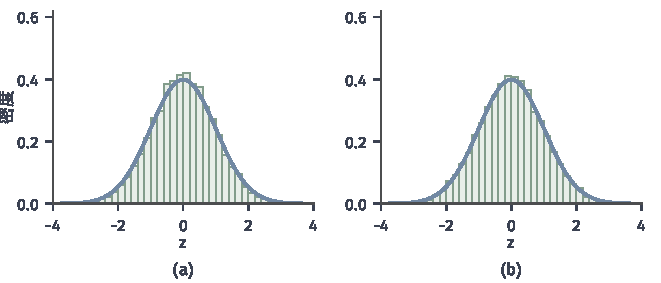
\includegraphics[width=112mm]{figures/07-probability/03-probability-limits/matplotlib/clt-pareto-third/figure.pdf}
 \caption{对称Pareto单项（密度$\frac32\lvert x\rvert^{-4}$，$\lvert x\rvert\geq1$，方差$3$，三阶绝对矩无穷）的标准化和$S_n/\sqrt{3n}$的直方图（浅绿，$20000$次重复，种子$11$）与$\varphi$（蓝）。(a)$n=10$；(b)$n=1000$。}
 \label{fig:clt-pareto-third}
\end{BookInlineFigure}

这个例子与第~\ref{sec:clt-lyapunov}节的比较是同一回事：收敛只看二阶矩，速度要看更高阶的矩。说“$n$足够大时可以用正态近似”之前，应当先问单项分布有没有有限的三阶矩，比值$\rho/\sigma^3$有多大，以及要计算的是典型区间的概率还是罕见事件的概率。


\section{本章小结}
\label{sec:clt-summary}

本章从掷硬币的正面次数出发，问许多独立小项之和的波动服从什么规律。第一步是选对中心和尺度：部分和的典型偏差按$\sigma\sqrt{n}$增长，平均的典型偏差按$\sigma/\sqrt{n}$缩小，只有放大$\sqrt{n}$倍的平均偏差才有不退化也不发散的极限。大数律确定了中心，中心极限定理刻画的是放大以后的形状；标准化只把均值和方差固定为$0$和$1$，形状接近钟形是独立求和的结果，特制硬币的Poisson极限说明了这一点。

在独立同分布、方差有限且为正的条件下，标准化部分和依分布趋于$\mathcal{N}(0,1)$。证明把和的特征函数写成$n$个相同因子的乘积：独立性给出乘积，中心化消去一次项，方差为一固定二次项，二阶矩有限经支配收敛使累计余项可以忽略，连续性定理把特征函数的收敛变回分布的收敛。各项分布不同时，以行内总方差$s_n^2$归一化，Lindeberg条件要求大值贡献的方差份额趋于零；Lyapunov条件用$2+\delta$阶矩换来更方便的核验。这些都是充分条件，各项为高斯而最大项占一半方差的例子说明它们不是必要的。

随机向量的情形由方向投影化为标量：正方差方向用标量定理，零方差方向的投影几乎必然为零，再由Cramér--Wold判据合成协方差为$\bm{\Sigma}$的联合高斯极限，$\bm{\Sigma}$可以奇异。骰子频率的极限就是一个集中在超平面上的退化高斯分布。

\begin{BookInlineTable}
 \centering
 \caption{本章的高斯极限与误差界}
 \label{tab:clt-summary}
 \begin{tabular}{lll}
 \toprule
 结论 & 对象 & 条件 \\
 \midrule
 定理~\ref{thm:clt-iid} & $Z_n$ & 独立同分布，$0<\sigma^2<\infty$ \\
 定理~\ref{thm:clt-lindeberg} & $S_n/s_n$ & 行内独立，Lindeberg条件 \\
 定理~\ref{thm:clt-lyapunov} & $S_n/s_n$ & 行内独立，$\Lambda_n(\delta)\to0$ \\
 定理~\ref{thm:clt-multivariate} & $\sqrt{n}(\bar{\bm{X}}_n-\bm{\mu})$ & 独立同分布，二阶矩有限 \\
 定理~\ref{thm:clt-berry-esseen} & $D_n\leq C\rho/(\sigma^3\sqrt{n})$ & 独立同分布，$\rho<\infty$ \\
 \bottomrule
 \end{tabular}
\end{BookInlineTable}

极限的存在不等于有限样本的精度。Berry--Esseen界在三阶绝对矩有限时给出对所有阈值一致的绝对误差$C\rho/(\sigma^3\sqrt{n})$，速度$1/\sqrt{n}$在格点分布上不能改进；对光滑的分布它可能偏保守。它不控制小尾概率的相对误差，偏斜分布在三四个标准差以外的尾概率可以与高斯近似相差数十倍；三阶矩无穷时，定理仍然成立，误差界却无从调用。

使用这些结论时，先确认中心与尺度，再看独立结构是同分布、三角阵还是向量，然后按要回答的问题核对矩条件：只问极限，二阶矩或Lindeberg条件就够了；要给定样本量下的误差，需要三阶矩；要罕见事件的概率，应回到精确分布或指数矩上界。第~\ref{chap:monte-carlo-integration-error}章将用本章的结论描述独立Monte Carlo积分的误差。

